% !TEX root = handbook-physics.tex
% !TEX TS-program = pdflatex
% !TEX encoding = UTF-8 Unicode






\chapter{Interference of Light}
\label{ch-32}
\zhtitle{光的干涉}

\section{Monochromaticity and Time Coherence of Light}
\label{sec-32.1} 
\zhtitle{光的单色性与时间相干性}

\subsection{}\label{32.1.1} \redem{Optics} is the branch of physics concerned with the study of the nature of light \ssect{31.4.3}, the laws of its production, propagation
and interaction with matter. Wave optics deals with optical
phenomena in which the wave nature of light is manifested
(for instance, interference, diffraction, polarization and dispersion of light). Since light comprises electromagnetic waves, wave optics is based on Maxwell's equations \ssect{27.4.3} and the relations that follow from them for electromagnetic waves (Section \ref{sec-31.1}).
\zhpar{\redem{光学}是研究光的本性、光的产生规律、光的传播及其与物质相互作用的物理学分支。波动光学研究光的波动性质所表现出的光学现象（例如光的干涉、衍射、偏振和色散）。由于光是电磁波，波动光学以麦克斯韦方程组（\ssect{27.4.3}）以及由其导出的电磁波关系（参见 \ref{sec-31.1} 节）为基础。}

Classical wave optics deals with media that are linear with
respect to their optical properties \ssect{30.1.7}, i.e. media in which the dielectric constant er and the magnetic permeability $\mu_{r}$ are independent of the intensity of the light \ssect{31.2.4}. Consequently, the principle of superposition \ssect{30.4.1} is valid in wave optics.
\zhpar{经典波动光学研究的是光学性质呈线性的介质（\ssect{30.1.7}），即相对电容率 $\varepsilon_{r}$ 和磁导率 $\mu_{r}$ 与光强无关的介质（\ssect{31.2.4}）。因此，叠加原理（\ssect{30.4.1}）在波动光学中成立。}

Phenomena that are observed in the propagation of light in
nonlinear media are investigated in \redem{nonlinear optics}. Nonlinear optical effects become appreciable at the very high intensities of light radiated by powerful lasers \ssect{39.8.8}.
\zhpar{研究光在非线性介质中传播时所观察到的现象，属于\redem{非线性光学}的内容。非线性光学效应只有在强激光器所辐射的极高光强下才变得显著（\ssect{39.8.8}）。}

\subsection{}\label{32.1.2} It has been experimentally established that the effect of light on a photocell, photographic film, fluorescent screen or other devices that record light is determined by the \redem{electric vector} $\vb{E}$ of the electromagnetic field set up by the light wave.
The same conclusion is reached by classical electronic theory,
according to which the processes caused in matter by light are
associated with the effect of the field of the light wave on charged particles of matter, i.e. on the electrons and ions. The frequency of visible and more short-waved light is so high $(\nu \gtrsim \SI{d15}{\hertz})$ that only electrons can execute forced vibration anywhere near appreciable in amplitude. 
\zhpar{光电池、照相胶片、荧光屏及其他记录光的器件，其响应取决于光波所建立的电磁场的\redem{电矢量} $\vb{E}$。经典电子理论也得出同样的结论：光在物质中引起的各种过程，与光波电场作用于物质中的带电粒子（即电子和离子）有关。可见光及比它频率更高的光，其频率是如此之高（$(\nu \gtrsim \SI{d15}{\hertz})$），以至于只有电子能够做出幅度明显的受迫振动。}

The force exerted by the electromagnetic
field \ssect{24.1.5} on an electron is
\zhpar{电磁场（\ssect{24.1.5}）作用于电子上的力为：}
\begin{equation*}%
\vb{F} = - e (\vb{E} + [\vb{v}_{1}\cross \vb{B}])  = -e (\vb{E} + \mu_{r}\mu_{0} [\vb{v}_{1}\cross \vb{H}]) .
\end{equation*}
Where $-e$ and $\vb{v}_{1}$ are the charge and velocity of the electron, and $\vb{B} = \mu_{r}\mu_{0}\vb{H}$ is the vector of magnetic induction. It follows from \ssect{31.1.5} that the absolute value of the magnetic component of force $\vb{F}$ is substantially less than its electrical component.
\zhpar{式中 $-e$ 与 $\vb{v}_{1}$ 分别为电子的电荷与速度，$\vb{B} = \mu_{r}\mu_{0}\vb{H}$ 为磁感应强度矢量。由\ssect{31.1.5}可知，力 $\vb{F}$ 的磁力分量的绝对值远小于其电力分量。}

Thus
\zhpar{因此有：}
\begin{equation*}%
\mu_{r}\mu_{0} [\vb{v}_{1}\cross \vb{H}] \leqslant \mu_{r}\mu_{0} {v}_{1}H = \frac{v_{1}}{v} E \ll E \qand \vb{F} \approx -e \vb{E},
\end{equation*}
because the velocity of electromagnetic waves is $v \approx  \SI{d8}{\meter\per\second}$, and the velocity of the electron in the atom upon forced vibrations set up by light is $v_{1} \approx \SI{d6}{\meter\per\second}$.
\zhpar{这是因为电磁波的速度 $v \approx \SI{d8}{\meter\per\second}$，而光致受迫振动时原子中电子的速度 $v_{1} \approx \SI{d6}{\meter\per\second}$。}

\subsection{}\label{32.1.3} In superposing light from two nonlaser sources\sidenote{This refers to ordinary light sources (incandescent lamps, discharge lamps, electric arcs, etc.), based on the principle of spontaneous radiation \ssect{39.8.6}} (for instance, two identical gas-discharge lamps), or even from different portions of the same source, no interference \ssect{30.5.2} is observed. Consequently, independent sources of light are incoherent \ssect{30.5.1} and their radiation is non-monochromatic
\ssect{31.1.6}. 
\zhpar{将两个非激光光源（例如两个相同的气体放电灯）发出的光叠加，甚至将同一光源不同部分发出的光叠加，都观察不到干涉（\ssect{30.5.2}）。因此，独立光源是非相干的（\ssect{30.5.1}），其辐射是非单色的（\ssect{31.1.6}）。}
\zhpar{注：此处指普通光源（白炽灯、放电灯、电弧灯等），其发光基于自发辐射原理（\ssect{39.8.6}）。}

The reason for this resides in the very mechanism by which light is radiated by the atoms (or molecules or ions) of the source. The excited atom radiates during an extremely
short de-excitation time, of the order of $\tau \approx \SI{d-8}{\second}$ \ssect{31.3.4}, after which it returns to its normal (unexcited) state, having expended its surplus energy on radiation. Following a certain period of time the atom may again be excited, obtaining energy externally, and begin to emit radiation again. Such intermittent radiation of light by atoms in the form of separate short impulses -- \redem{wave trains}, or \redem{packets} -- is typical of any light source, regardless of the specific processes that occur in the source and excite its atoms. In spontaneous radiation \ssect{39.8.6}, the atoms emit radiation independently of one another with random initial phases that vary without any order from one event of emission to another. Therefore, spontaneously radiating atoms are incoherent sources of light.
\zhpar{其原因在于光由光源中的原子（或分子、离子）辐射的机制本身。受激发的原子在极短的退激时间内发光，其量级为 $\tau \approx \SI{d-8}{\second}$（\ssect{31.3.4}），之后回到正常（未激发）状态，并将多余的能量以辐射形式释放。经过一段时间后，原子可能再从外界获得能量而重新被激发，并再次发光。原子以一段段彼此分立的短脉冲形式间歇地发光——这些脉冲称为\redem{波列}，或\redem{波包}——这是任何光源的共同特征，与光源中发生的具体过程以及激发原子的方式无关。在自发辐射（\ssect{39.8.6}）中，各原子彼此独立地发光，其初相位是随机的，并且在每次发射之间无序地变化。因此，自发辐射的原子是非相干的光源。}


Induced, or stimulated, emission of radiation is quite
another matter. It is produced in a nonequilibrium (active)
medium by the action of a variable electromagnetic field \ssect{39.6.1}. Stimulated emission of radiation by all the particles of a system is coherent with the monochromatic radiation that it is produced by, having the same frequency, polarization and direction of propagation. These features of stimulated emission of radiation are made use of in lasers and masers \ssect{39.8.8}.
\zhpar{感应辐射，即受激辐射，则完全是另一回事。它是在非平衡（激活）介质中，由变化的电磁场作用（\ssect{39.6.1}）而产生的。受激辐射时，系统中所有粒子所发出的辐射都与产生它的单色辐射相干，具有相同的频率、偏振和传播方向。激光器和微波激射器正是利用了受激辐射的这些特性（\ssect{39.8.8}）。}

\subsection{}\label{32.1.4} A real wave, radiated during a limited period of time and encompassing a limited region of space, is not monochromatic. The spectrum of its angular frequencies \ssect{28.4.7} is of finite width $\Delta \omega$, i.e. it includes angular frequencies from $ \omega - \Delta  \omega/2$ to $ \omega + \Delta  \omega/2$. During the time interval $\Delta t \ll = \tau_{coh} = \pi/ \Delta \omega$
such a wave can be considered as an approximately monochromatic wave with the angular frequency $\omega$. 
\zhpar{实际的波是在有限时间内辐射、并占据有限空间区域的，因此不是单色波。其角频率谱（\ssect{28.4.7}）具有有限的宽度 $\Delta \omega$，即包含从 $\omega - \Delta \omega/2$ 到 $\omega + \Delta \omega/2$ 之间的角频率。在时间间隔 $\Delta t \ll = \tau_{coh} = \pi/ \Delta \omega$ 内，这种波可以近似地看作角频率为 $\omega$ 的单色波。}

The quantity $\tau_{coh}$ is called the \redem{time coherence of a nonmonochromatic wave}. During the time interval $\tau_{coh}$ the phase difference of the vibrations corresponding to waves of the frequencies $ \omega + \Delta  \omega/2$ and $ \omega +-\Delta  \omega/2$ changes by $\pi$. A wave with the angular frequency co and phase velocity $v$ propagates during this time over the distance $l_{coh} =  \tau_{coh} = \pi v/\Delta \omega$.
\zhpar{量 $\tau_{coh}$ 称为\redem{非单色波的时间相干性}。在时间间隔 $\tau_{coh}$ 内，频率为 $\omega + \Delta \omega/2$ 与 $\omega +-\Delta \omega/2$ 的波所对应的振动，其相位差改变 $\pi$。角频率为 $\omega$、相速度为 $v$ 的波，在这段时间内所传播的距离为 $l_{coh} = \tau_{coh} = \pi v/\Delta \omega$。}

The quantity $l_{coh}$ is called the \redem{coherence length}, or the \redem{harmonic wave train length}, of the corresponding nonmonochromatic wave being considered. The closer a given wave is to a monochromatic one, the less the width $\Delta \omega$ of its frequency spectrum and the greater its coherence time and coherence length. For example, for visible sunlight, having a continuous frequency spectrum from \num{4d14} to \SI{8d14}{\hertz}, $\tau_{coh} \approx \SI{d-14}{\second}$ and $l_{coh} \approx \SI{d-8}{\meter}$. The coherence time of stimulated radiation is substantially longer than the de-excitation time of the atom \ssect{31.3.4}. For example, $\tau_{coh}$ reaches \SI{d-5}{\second} for a continuous-wave laser and the coherence length $l_{coh} \approx \SI{d3}{\meter}$.
\zhpar{量 $l_{coh}$ 称为相应非单色波的\redem{相干长度}，或称\redem{简谐波列长度}。波越接近单色波，其频谱宽度 $\Delta \omega$ 越小，相干时间与相干长度就越大。例如，对于频谱连续、范围从 \num{4d14} 到 \SI{8d14}{\hertz} 的可见太阳光，$\tau_{coh} \approx \SI{d-14}{\second}$，$l_{coh} \approx \SI{d-8}{\meter}$。受激辐射的相干时间远长于原子的退激时间（\ssect{31.3.4}）。例如，对于连续波激光器，$\tau_{coh}$ 可达 \SI{d-5}{\second}，相干长度 $l_{coh} \approx \SI{d3}{\meter}$。}

\section{Interference of Light. Spatial Coherence of Light}
\label{sec-32.2} 
\zhtitle{光的干涉。光的空间相干性}


\subsection{}\label{32.2.1} To obtain coherent light waves by means of conventional
(nonlaser) light sources, light from a single source is split into two or more systems of waves. Each system represents the
radiation of the same atoms of the source. Hence, by virtue of
their common origin, these systems of waves are coherent with
one another and interfere when superposed. Light can be split
into coherent systems of waves by its reflection or refraction.
\zhpar{要用普通（非激光）光源获得相干光波，需将单一光源发出的光分成两束或更多的波系。每一波系都代表光源中同一批原子的辐射。因此，由于它们具有共同的起源，这些波系彼此相干，叠加时会发生干涉。光可以通过反射或折射而分成相干的波系。}
\begin{marginfigure}[-3cm]
\centering
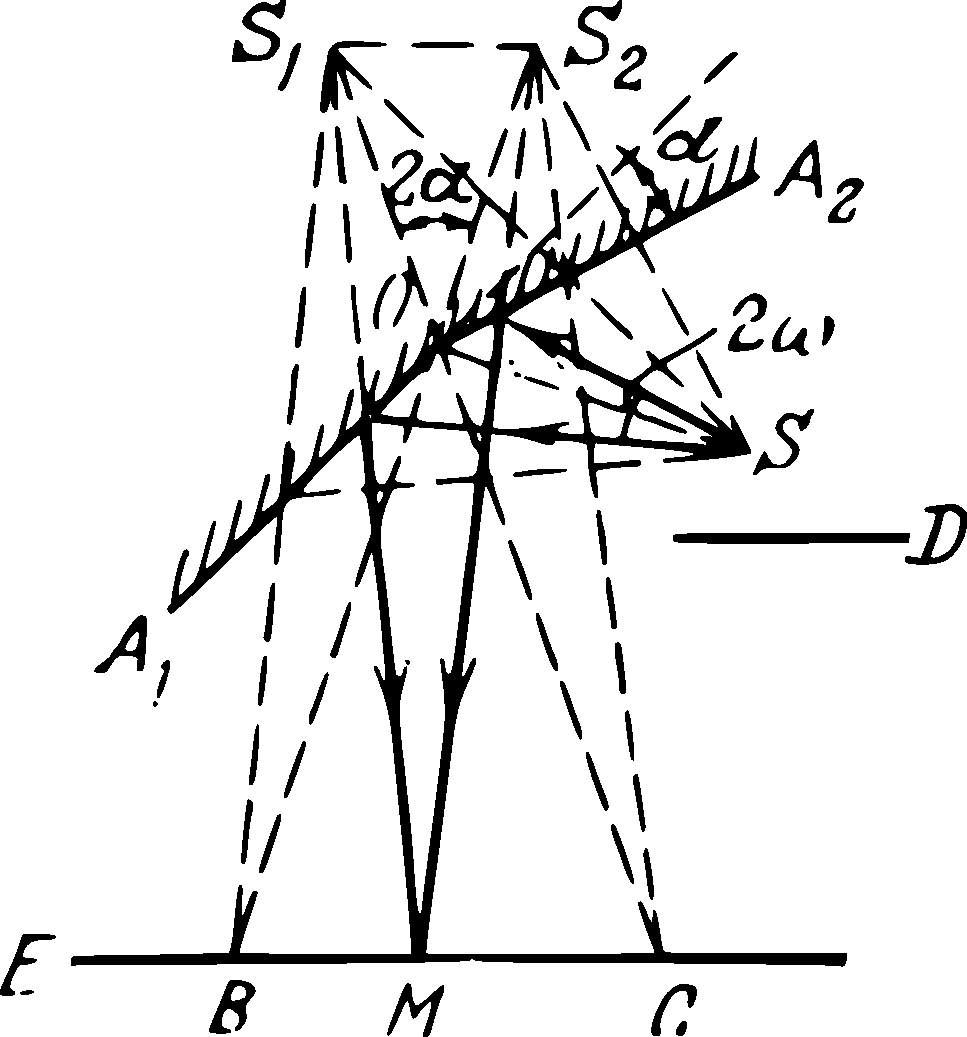
\includegraphics[width=\textwidth]{figs/ch-32/fig-32-01.pdf}
\sidecaption{Fresnel mirrors and interference of light.\zhcap{菲涅耳双镜与光的干涉。}\label{fig-32-01}}
\end{marginfigure}
Illustrated as an example in \figr{fig-32-01} is the principle of the \redem{Fresnel mirrors}. Light from point source S is incident on two plane mirrors $A_{1}O$ and $A_{1}O$ arranged perpendicular to the plane of the drawing and joined along line $O$. The angle $\alpha$ be tween the planes of the mirrors is very small. Light from source $S$ propagates after being reflected as two beams having their centres at points $S_{1}$ and $S_{2}$, which are the virtual images of source S in the mirrors. These beams are coherent and upon being superposed produce an interference pattern on screen $E$ (the region $BC$ is sometimes called the \redem{field of interference}). The result of the interference at some point $M$ on the screen depends upon the wavelength $\lambda$ of the light and the path difference of the waves \ssect{30.5.2} from
the coherent virtual sources and $S_{2}$ to point $M$. 
\zhpar{以\figr{fig-32-01}为例，说明\redem{菲涅耳双镜}的原理。来自点光源 $S$ 的光入射到两个平面镜 $A_{1}O$ 与 $A_{2}O$ 上，两镜垂直于图面，并沿直线 $O$ 相接。两镜面之间的夹角 $\alpha$ 很小。光源 $S$ 发出的光经两镜反射后形成两束光，其中心分别位于两点 $S_{1}$ 与 $S_{2}$，它们是光源 $S$ 在两镜中所成的虚像。这两束光是相干的，叠加后在屏 $E$ 上形成干涉图样（区域 $BC$ 有时称为\redem{干涉场}）。屏上某点 $M$ 处的干涉结果，取决于光的波长 $\lambda$，以及从相干虚光源 $S_{1}$ 和 $S_{2}$ 到点 $M$ 的波的波程差（\ssect{30.5.2}）。}

Thus,
\zhpar{由此得：}
\begin{equation*}%
\Delta = r_{2} - r_{1} = \overline{MS_{2}} - \overline{MS_{1}}.
\end{equation*}
\begin{marginfigure}%[-3cm]
\centering
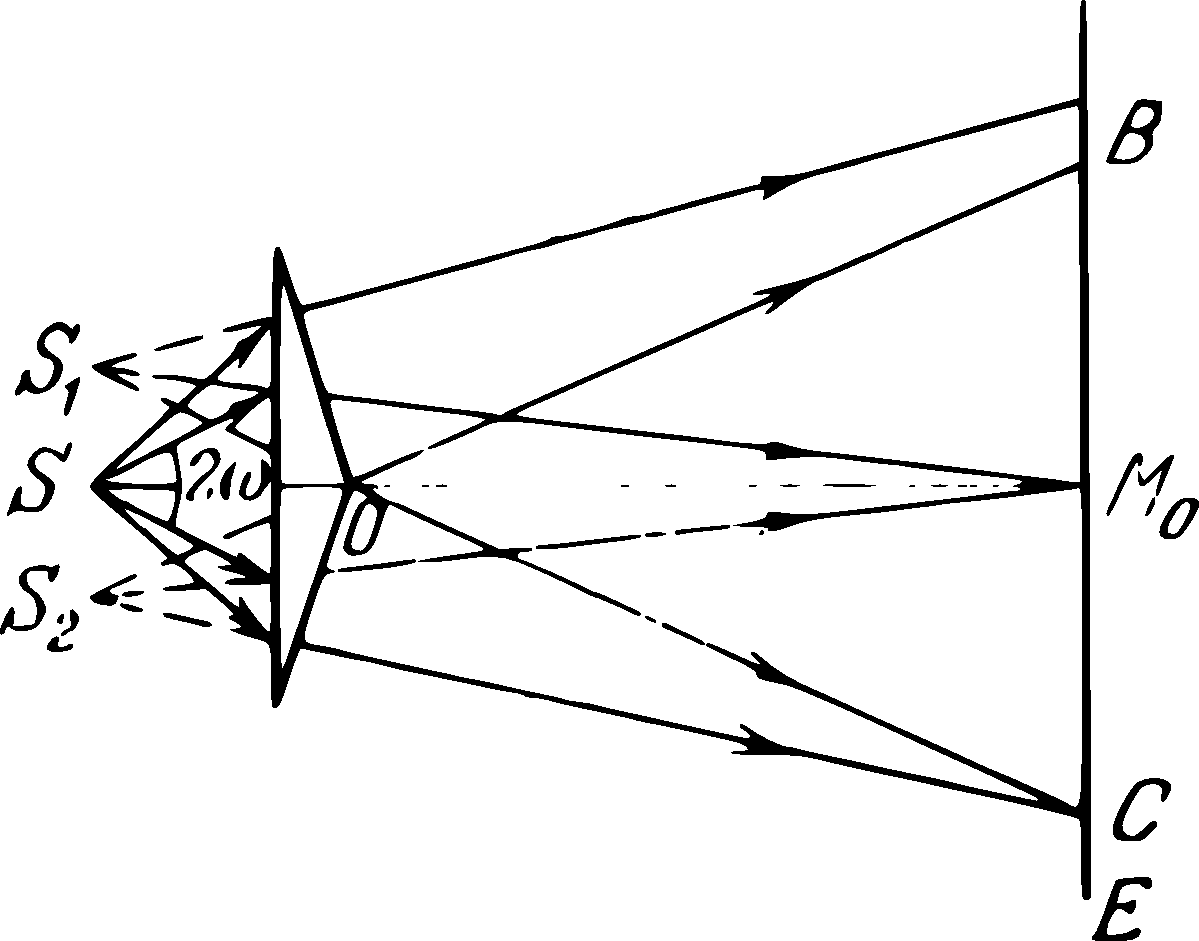
\includegraphics[width=\textwidth]{figs/ch-32/fig-32-02.pdf}
\sidecaption{the Fresnel biprism.\zhcap{菲涅耳双棱镜。}\label{fig-32-02}}
\end{marginfigure}
The initial phases of vibration of sources $S_{1}$ and $S_{2}$ are the same. Hence, the \redem{conditions for interference maxima and minima} \ssect{30.5.2} are of the form
\zhpar{虚光源 $S_{1}$ 与 $S_{2}$ 的振动初相位相同。因此，干涉极大与极小的条件（\ssect{30.5.2}）具有如下形式：}
\begin{equation*}%
 r_{2} - r_{1} = \pm m\,\lambda,
\end{equation*}
for a maximum of the $m$-th order $(m = 0, \,1,\, 2, \dots)$,
\zhpar{对于第 $m$ 级极大（$m = 0, \,1,\, 2, \dots$），}
\begin{equation*}%
 r_{2} - r_{1} = \pm \, (2m - 1) \frac{\lambda}{2},
\end{equation*}
for a minimum of the $m$-th order $(m = 0, \,1,\, 2, \dots)$.
\zhpar{对于第 $m$ 级极小（$m = 0, \,1,\, 2, \dots$）。}

The angle $2\omega$ at apex $S$ between the two rays of light that converge at point $M$ of the interference pattern after being reflected from mirrors $A_{1}O$ and $A_{2}O$ is called the \redem{aperture angle of the interference}. This angle usually varies very little upon changing the position of point $M$ within the limits of the field of interference.
\zhpar{在光源 $S$ 处，两条分别经镜面 $A_{1}O$ 与 $A_{2}O$ 反射后会聚于干涉图样中点 $M$ 的光线所夹的角 $2\omega$，称为\redem{干涉孔径角}。在干涉场内改变点 $M$ 的位置时，该角度通常变化很小。}
\begin{marginfigure}%[-3cm]
\centering
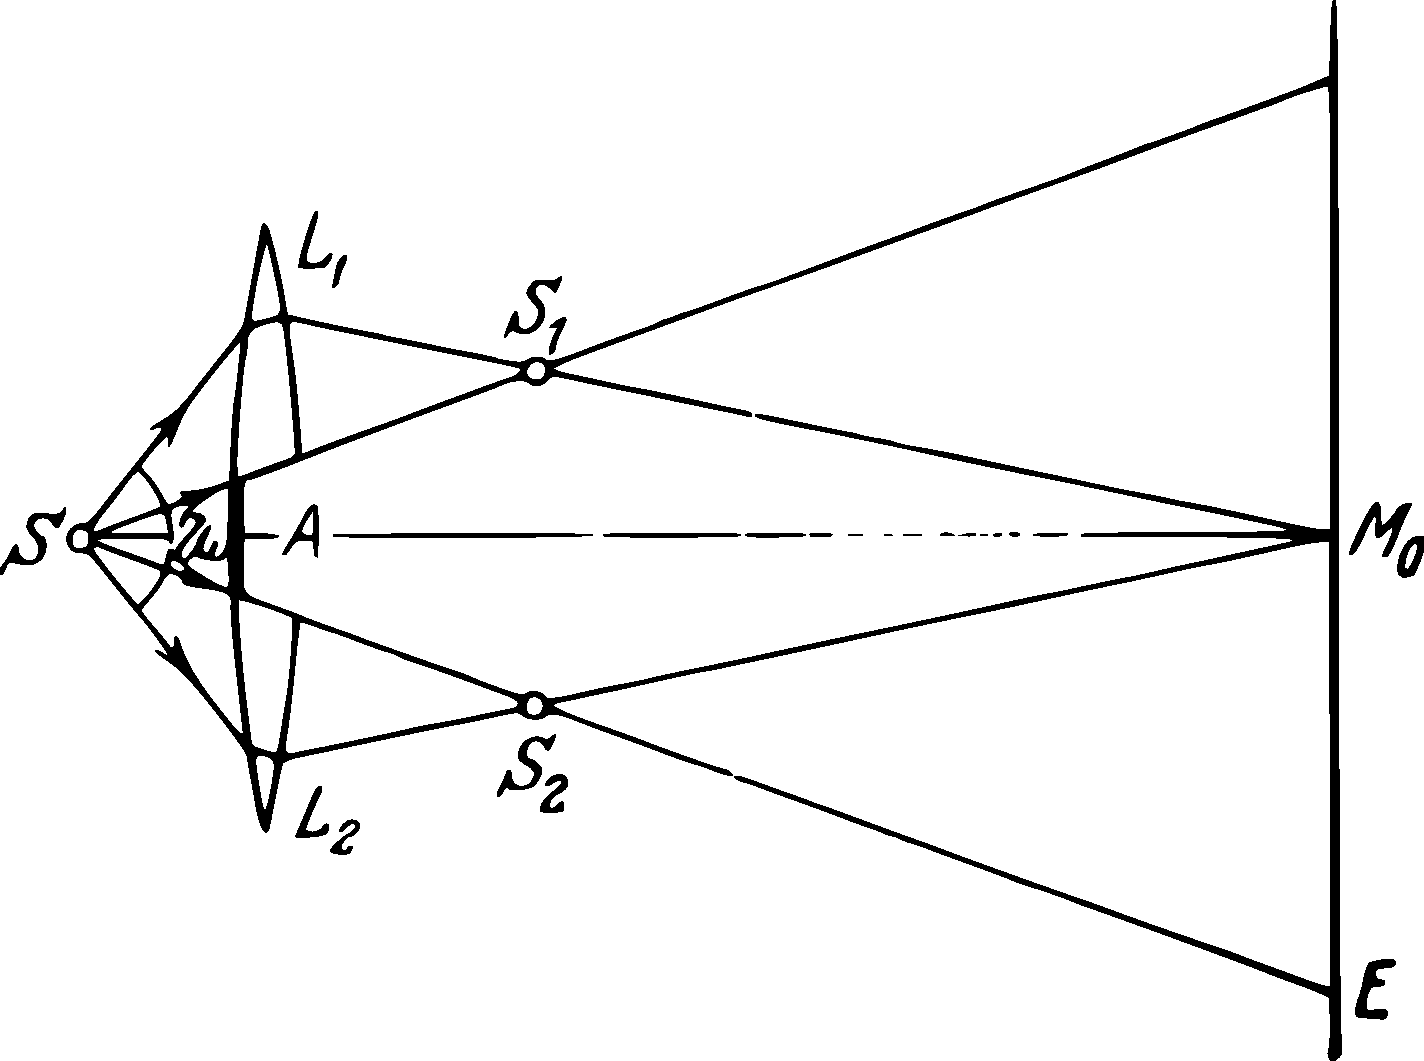
\includegraphics[width=\textwidth]{figs/ch-32/fig-32-03.pdf}
\sidecaption{Billet split lens.\zhcap{比累分割透镜。}\label{fig-32-03}}
\end{marginfigure}

\subsection{}\label{32.2.2} The principles of the techniques used for observing interference by means of the \redem{Fresnel biprism} (\figr{fig-32-02}) and the \redem{Billet split lens} ( \figr{fig-32-03}) are similar to those of the Fresnel mirrors. The biprism consists of two identical triangular prisms joined together at their bases and prepared as a whole. The refracting angles a at the upper and lower edges of the biprism are very small (of the order of a fraction of one degree). 
\zhpar{利用\redem{菲涅耳双棱镜}（\figr{fig-32-02}）和\redem{比累分割透镜}（\figr{fig-32-03}）观察干涉的技术原理，与菲涅耳双镜相似。双棱镜由两个相同的三棱镜沿底边贴合而成。双棱镜上、下两侧棱边处的折射角 $\alpha$ 都很小（约为一度的几分之一）。}

Light from source $S$ is refracted in the biprism and propagates in it in the form of two systems of waves, corresponding to the coherent virtual sources of light $S_{1}$ and $S_{2}$. The interference of these waves is observed in the region of their overlapping on screen $E$.
\zhpar{光源 $S$ 发出的光经双棱镜折射后，以两个波系的形式在棱镜中传播，这两个波系分别对应于相干虚光源 $S_{1}$ 与 $S_{2}$。这些波在屏 $E$ 上相互交叠的区域中发生干涉。}

The Billet split lens consists of two halves $L_{1}$ and $L_{2}$ of a collecting lens, cut along a diameter. The two halves are slightly displaced laterally (spread apart). In consequence, they produce two noncoinciding real images $S_{1}$ and $S_{2}$ of the point source of light $S$. The interference of light from these coherent secondary sources is observed on screen $E$. The space between parts $L_{1}$ and $L_{2}$ of the split lens is covered by opaque screen $A$.
\zhpar{比累分割透镜由一个会聚透镜沿直径剖开得到的两半 $L_{1}$ 与 $L_{2}$ 构成。两半透镜略微横向错开（彼此分开），因此对点光源 $S$ 形成两个不重合的实像 $S_{1}$ 与 $S_{2}$。这两个相干次级光源发出的光在屏 $E$ 上产生干涉。分割透镜的两半 $L_{1}$ 与 $L_{2}$ 之间的空隙，由不透光屏 $A$ 遮挡。}

The value of the aperture angle $2\omega$ of interference is shown in \figr{fig-32-02} and \figr{fig-32-03} for the central point $M_{0}$ of the interference pattern obtained by means of a biprism and a split lens.
\zhpar{干涉孔径角 $2\omega$ 的数值在\figr{fig-32-02}与\figr{fig-32-03}中给出，分别对应于双棱镜和分割透镜所得干涉图样的中心点 $M_{0}$。}

\subsection{}\label{32.2.3} The \redem{width of an interference fringe} (as the bands are called) is the distance between two adjacent interference maxima (or minima). When the Fresnel mirrors or similar devices (biprisms or split lenses) are employed to obtain interference, the width of an interference fringe \ssect{30.5.2} is $\lambda L/l$. Here $l$ is the distance between sources $S_{1}$ and $S_{2}$, and $L$ is the distance from them to screen $E$. The wavelength of visible light is extremely short $(\lambda \approx \SI{5d-7}{\meter})$. Therefore, to obtain an interference fringe of a width that can be resolved by the eye, it is necessary
to comply with the condition: $l \ll L$. Consequently, the angle $\alpha$ in the Fresnel mirrors and the refracting angles $\alpha$ of the biprism must be very small.
\zhpar{\redem{干涉条纹的宽度}（条纹亦称条带）是指相邻两个干涉极大（或极小）之间的距离。采用菲涅耳双镜或类似装置（双棱镜或分割透镜）获得干涉时，条纹宽度为 $\lambda L/l$。其中 $l$ 为两光源 $S_{1}$ 与 $S_{2}$ 之间的距离，$L$ 为它们到屏 $E$ 的距离。可见光的波长极短（$\lambda \approx \SI{5d-7}{\meter}$）。因此，要得到人眼能够分辨的条纹宽度，必须满足条件：$l \ll L$。由此可知，菲涅耳双镜中的角 $\alpha$ 以及双棱镜的折射角 $\alpha$ 必须很小。}

The possibility of observing interference fringes also depends on the \redem{degree of contrast}, i.e. on the degree of different illumination of the screen at the maxima and minima. The illuminance is proportional to the intensity $I$ of the incident light. A quantitative characteristic of the degree of contrast of the interference pattern is the dimensionless quantity called the \redem{visibility of fringes}:
\zhpar{能否观察到干涉条纹还取决于\redem{对比度}，即屏上干涉极大处与极小处照度的差异程度。照度与入射光强度 $I$ 成正比。干涉图样对比度的定量特征是一个无量纲量，称为\redem{条纹可见度}，其定义如下式所示：}
\begin{equation*}%
V = \frac{I_{\text{max}} - I_{\text{min}}}{I_{\text{max}} + I_{\text{min}}},
\end{equation*}
where $I_{\text{max}}$ and $I_{\text{min}}$ are the values of the light intensities in the interference maxima and minima on the screen. The human eye reliably distinguishes fringes if their visibility $V > 0.1$, i.e. when $I_{\text{min}} < 0.82 I_{\text{max}}$.
\zhpar{式中 $I_{\text{max}}$ 与 $I_{\text{min}}$ 分别为屏上干涉极大与极小处的光强。当条纹可见度 $V > 0.1$，即 $I_{\text{min}} < 0.82 I_{\text{max}}$ 时，人眼才能可靠地分辨条纹。}

In superposing two likewise polarized coherent monochromatic
waves, with the amplitudes and intensities $A_{1}$, $I_{1}$, $A_{2}$ and $I_{2}$, the visibility of the fringes is
\zhpar{将两束偏振方向相同、相干的单色波叠加时，它们的振幅与强度分别为 $A_{1}$、$I_{1}$、$A_{2}$ 和 $I_{2}$，此时条纹可见度为：}
\begin{equation*}%
V = \frac{2A_{1}A_{2}}{A_{1}^{2}+A_{2}^{2}} = \frac{2 \sqrt{I_{1}I_{2}}}{I_{1} + I_{2}}.
\end{equation*}
The visibility of theiringes is a maximum $(V = 1)$ when $A_{1} = A_{2}$.
\zhpar{当 $A_{1} = A_{2}$ 时，条纹可见度最大（$V = 1$）。}

\subsection{}\label{32.2.4} In an interference arrangement of the type of the Fresnel mirrors, illuminated by a point source $S$ (\figr{fig-32-01}), the superposed waves are never ideally monochromatic \ssect{32.1.3}. Hence, these waves are only \redem{partly coherent}. They are capable of interference
only under the condition that the vibration, excited by
them at point $M$ being considered on the screen, corresponds to one and the same harmonic train, or packet, of radiation of
source $S$ \ssect{32.1.4} i.e. if
\zhpar{在点光源 $S$ 照明的菲涅耳双镜型干涉装置中（\figr{fig-32-01}），被叠加的波永远不可能是理想单色的（\ssect{32.1.3}）。因此，这些波只是\redem{部分相干的}。只有当它们在屏上所考察的点 $M$ 处激发的振动，对应于光源 $S$ 发出的同一个简谐波列或波包（\ssect{32.1.4}）时，它们才能发生干涉，即满足下式：}
\begin{equation*}%
\abs{r_{2} - r_{1} } < v \tau_{\text{coh}} \qor \abs{r_{2} - r_{1} } < l_{\text{coh}}.
\end{equation*}
Here $r_{2} - r_{1}$ is the path difference of the superposed waves, $v$ is their velocity, $\tau_{\text{coh}}$ and xc0h and $l_{\text{coh}}$ are coherence time and coherence length of light from source $S$ \ssect{32.1.4}. \redem{Partly coherent
vibrations are combined} at point $M$. These vibrations are excited by the same source $S$ at different instants of time, $t$ and $t + \tau$, where $\tau = \abs{ r_{2} - r_{1} }/v$. Therefore, the visibility of the interference pattern in such arrangements essentially depends on the \redem{time-coherence of the vibrations}, which is limited by the mono-chromaticity of the light from source $S$, i.e. its coherence time
Tcoh \ssect{32.1.4}. At $\tau \ll \tau_{\text{coh}}$ the superposed vibrations are practically fully coherent and the visibility of the interference fringes (at equal intensity of the superposed waves) $V \approx 1$. If, however,
$\tau \geqslant \tau_{\text{coh}}$ the superposed vibrations are incoherent and there is no interference $(V = 0)$.
\zhpar{式中 $r_{2} - r_{1}$ 为被叠加波的波程差，$v$ 为其速度，$\tau_{\text{coh}}$ 与 $l_{\text{coh}}$ 为光源 $S$ 发出的光的相干时间与相干长度（\ssect{32.1.4}）。\redem{部分相干的振动}在点 $M$ 处叠加。这些振动由同一光源 $S$ 在不同时刻 $t$ 与 $t + \tau$ 激发，其中 $\tau = \abs{ r_{2} - r_{1} }/v$。因此，这类装置中干涉图样的可见度主要取决于\redem{振动的时间相干性}，而时间相干性受光源 $S$ 发出的光的单色性限制，即受其相干时间 $\tau_{\text{coh}}$ 限制（\ssect{32.1.4}）。当 $\tau \ll \tau_{\text{coh}}$ 时，被叠加的振动实际上完全相干，若被叠加波的强度相等，则条纹可见度 $V \approx 1$。然而，若 $\tau \geqslant \tau_{\text{coh}}$，被叠加的振动不相干，不发生干涉（$V = 0$）。}

Thus, to observe the interference of light at large path differences $r_{2} - r_{1}$ (and corresponding large values of $\tau$) it is necessary for the light to have a sufficiently long coherence time, i.e. a sufficiently high degree of monochromaticity.
\zhpar{因此，要在较大的波程差 $r_{2} - r_{1}$（以及相应较大的 $\tau$）下观察光的干涉，光必须具有足够长的相干时间，即具有足够高的单色性。}

\subsection{}\label{32.2.5} The positions on the screen of all the interference maxima, with the exception of the zero-order maximum, depend upon the wavelength of the light. For two wavelengths $\lambda_{1}$ and $\lambda_{2}$, the higher the order $m$ to be observed, the more their maxima of the $m$-th order are displaced from each other. Therefore, as $m$ is
increased, the visibility of interference fringes, obtained by the illumination of Fresnel mirrors with nonmonochromatic light, is impaired. Fringes, corresponding to different values of $\lambda$, are superposed on one another, and the interference pattern is blurred.
\zhpar{除零级极大外，屏上所有干涉极大的位置都与光的波长有关。对于两个波长 $\lambda_{1}$ 与 $\lambda_{2}$，所观察的级次 $m$ 越高，它们的第 $m$ 级极大彼此错开得越远。因此，随着 $m$ 增大，用非单色光照明菲涅耳双镜所得干涉条纹的可见度会下降。对应于不同 $\lambda$ 值的条纹彼此叠加，干涉图样变得模糊。}


Assume that the wavelength of light is within the limits from $\lambda$ to $\lambda + \Delta \lambda$, and the angular frequency, from $\omega$ to $\omega - \Delta \omega$,
where $\Delta \omega = 2 \pi v \Delta \lambda/ \lambda^{2}$. Then, according to the \redem{Rayleigh criterion}, the interference pattern is still distinguishable up to a maximum of the $m_{0}$ order for light with the wavelength $\lambda + \Delta \lambda$ (where $\Delta \lambda > 0$), which is superposed on the screen on the nearest interference minimum for light of wavelength $\lambda$:
\zhpar{设光的波长在 $\lambda$ 到 $\lambda + \Delta \lambda$ 之间变化，相应的角频率从 $\omega$ 到 $\omega - \Delta \omega$，其中 $\Delta \omega = 2 \pi v \Delta \lambda/ \lambda^{2}$。那么，根据\redem{瑞利判据}，对于波长为 $\lambda + \Delta \lambda$（$\Delta \lambda > 0$）的光，直到第 $m_{0}$ 级极大时干涉图样仍可分辨；该级极大恰好与波长为 $\lambda$ 的光的最近一个干涉极小重叠于屏上，即满足下式：}
\begin{align*}%
m_{0} (\lambda + \Delta \lambda) & = (2m_{0} +1) \frac{\lambda}{2}, \text{ from which}\\
m_{0} & = \frac{\lambda}{2 \Delta \lambda}.
\end{align*}
Thus, interference can be observed at path differences of the
waves that comply with the condition
\zhpar{因此，只有当波的波程差满足下列条件时，才能观察到干涉：}
\begin{equation*}%
\abs{r_{2} - r_{1}} \leqslant \frac{\lambda^{2}}{2\Delta  \lambda} =\frac{\pi v}{\Delta \omega} = v \tau_{\text{coh}}.
\end{equation*}
This result agrees with the assessment made in \ssect{32.2.4} on the basis of the concept of time coherence of vibrations.
\zhpar{这一结果与\ssect{32.2.4}中基于振动的时间相干性概念所作的估计一致。}

\subsection{}\label{32.2.6} Partly coherent light, of a total intensity $I$, can be dealt with as the combination of two components: the coherent component of intensity $\gamma I$, where $\gamma$ is the \redem{degree of coherence of the
light}, and the incoherent component of the intensity $(1-\gamma)I$.
\zhpar{总强度为 $I$ 的部分相干光，可以看作两个分量的叠加：强度为 $\gamma I$ 的相干分量，其中 $\gamma$ 为\redem{光的相干度}；以及强度为 $(1-\gamma)I$ 的非相干分量。}

When partly coherent waves are superposed, only their coherent
components interfere. The incoherent components produce the
uniformly illuminated background of the interference pattern.
Therefore, as the degree of coherence of the light is reduced, the visibility $V$ of the interference fringes decreases. Thus
\zhpar{部分相干的波叠加时，只有其相干分量发生干涉，非相干分量则在干涉图样中形成均匀照明的背景。因此，光的相干度降低时，干涉条纹的可见度 $V$ 随之减小。于是有：}
\begin{equation*}%
V = \frac{2 \sqrt{I_{1}I_{2}}}{I_{1}+ I_{2}} \, \gamma.
\end{equation*}
When the intensities of partly coherent waves are the same
$V = \gamma$.
\zhpar{当部分相干波的强度相等时，$V = \gamma$。}

\subsection{}\label{32.2.7} As a rule, in an interference device with mirrors (or a biprism), a brightly illuminated narrow slit, parallel to the joint $O$ between the mirrors, is used instead of a point source of light. In this case, the interference patterns, obtained on the screen from the various portions along the length of the slit, are displaced with respect to one another inthe direction of the slit $S$. Accordingly, a system of interference fringes, parallel
to joint $O$ of the mirrors, is observed on the screen.
\zhpar{通常，在镜面（或双棱镜）干涉装置中，用一条与镜面交线 $O$ 平行、被强烈照明的狭缝代替点光源。这时，屏上来自狭缝不同部分的干涉图样，沿狭缝方向 $S$ 彼此错开。因此，屏上观察到的是一组与镜面交线 $O$ 平行的干涉条纹。}

The visibility of the interference fringes is reduced as the width of the slit $S$ is increased. This is due to the fact that the interference fringes that could be obtained on the screen from various narrow slits into which slit $S$ could be conceivably divided would be displaced with respect to one another. An interference pattern in monochromatic light of wavelength $\lambda$ is sharp and distinct if the following approximate condition is complied with:
\zhpar{随着狭缝 $S$ 宽度的增大，干涉条纹的可见度降低。这是因为，若设想将狭缝 $S$ 分割成许多窄缝，各窄缝在屏上所得的干涉条纹会彼此错开。波长为 $\lambda$ 的单色光所形成的干涉图样清晰、分明的近似条件是：}
\begin{equation*}%
b \sin \omega \leqslant  \frac{\lambda}{4},
\end{equation*}
where $b$ is the slit width and $2 \omega$ is the aperture angle of interference \ssect{32.2.1}.
\zhpar{式中 $b$ 为狭缝宽度，$2 \omega$ 为干涉孔径角（\ssect{32.2.1}）。}
\begin{marginfigure}%[-3cm]
\centering
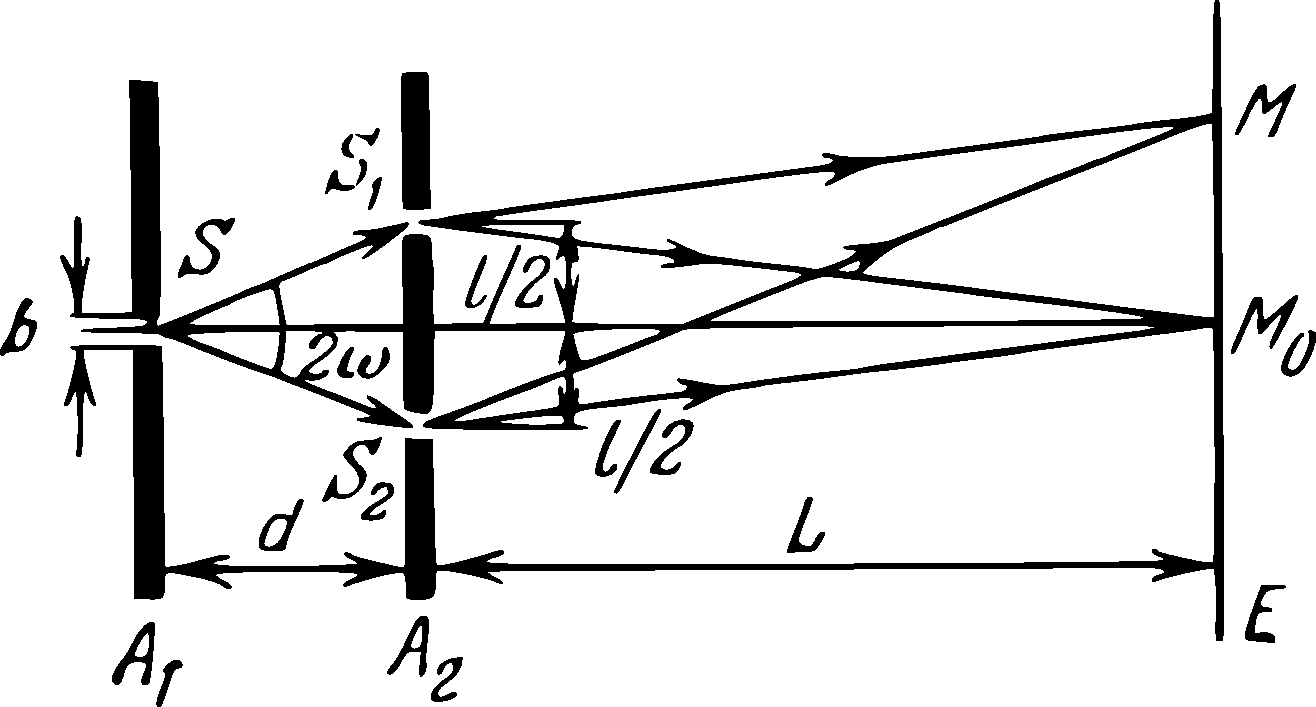
\includegraphics[width=\textwidth]{figs/ch-32/fig-32-04.pdf}
\sidecaption{Young's double-slit method for interference of light.\zhcap{光的杨氏双缝干涉法。}\label{fig-32-04}}
\end{marginfigure}

\subsection{}\label{32.2.8} The principle of \redem{Young's two-slit interference method} is illustrated in \figr{fig-32-04}. The source of light is a brightly illuminated
narrow slit $S$ in screen $A_{1}$. Light from slit $S$ falls on a second opaque screen $A_{2}$ having two identical narrow slits $S_{1}$ and $S_{2}$ parallel to slit $S$. Two systems of cylindrical waves are propagated in the space beyond screen $A_{2}$ their interference is observed on screen $E$. The visibility of the interference fringes for small path differences is determined mainly by the degree of agreement in the way the vibrations are executed at points of 
slits $S_{1}$ and $S_{2}$. These slits can be considered as the ``sources'' of the waves interfering on the screen.
\zhpar{\redem{杨氏双缝干涉法}的原理如\figr{fig-32-04}所示。光源是位于屏 $A_{1}$ 上、被强烈照明的狭缝 $S$。来自狭缝 $S$ 的光射到另一块不透光屏 $A_{2}$ 上，该屏上有两条与狭缝 $S$ 平行、完全相同的窄缝 $S_{1}$ 与 $S_{2}$。屏 $A_{2}$ 之后的空间中传播着两列柱面波，它们的干涉在屏 $E$ 上被观察到。对于较小的波程差，干涉条纹的可见度主要取决于狭缝 $S_{1}$ 与 $S_{2}$ 处各点振动的步调一致程度。这两条狭缝可看作屏上发生干涉的波的“波源”。}

\subsection{}\label{32.2.9} The coherence of vibrations executed at the same instant of time at various points of a plane $Q$, perpendicular to the direction of wave propagation, is called spatial coherence (as distinguished from time coherence of vibrations, executed at one and the same point, but at different instants of time).
\zhpar{在垂直于波传播方向的平面 $Q$ 上，同一时刻不同点处振动的相干性，称为\redem{空间相干性}（区别于同一点在不同时刻振动之间的时间相干性）。}

Spatial coherence depends upon the conditions for the radiation and formation of light waves. For instance, a light wave emitted by a point source has complete spatial coherence. In the case of an ideal plane wave, the amplitude and phase of the vibration are the same at all points, of plane $Q$, i.e. there is also complete spatial coherence. Spatial coherence is also maintained over the whole cross section of a light beam emitted by a laser.
\zhpar{空间相干性取决于光波辐射与形成的条件。例如，点光源发出的光波具有完全的空间相干性。对于理想平面波，平面 $Q$ 上各点的振动振幅和相位都相同，即同样具有完全的空间相干性。激光器发出的光束，其整个横截面上也都保持着空间相干性。}

In a real wave, emitted by a host of independent atoms of an
extended nonlaser light source, the phase difference of the
vibrations at two points $K_{1}$ and $K_{2}$ of plane $Q$ is a random function of time. The random variations of the phase difference increase with the distance between the points. The \redem{length of spatial coherence} is the distance $l_{sc}$ between points $K_{1}$ and $K_{2}$ of plane $Q$ at which the random changes of phase difference reach a value equal to it. 

If in Young's two-slit interference arrangement the distance $l$ between slits $S_{1}$ and $S_{2}$ is greater than or equal to $l_{sc}$ the visibility of the interference fringes equals zero. To ensure spatial coherence in the illumination of slits $S_{1}$ and $S_{2}$, the width $b$ of inlet slit $S$ should be sufficiently narrow. Thus
\zhpar{对于由大量彼此独立的原子发出的、具有一定延展尺寸的非激光光源所发出的实际波，平面 $Q$ 上两点 $K_{1}$ 与 $K_{2}$ 处振动的相位差是时间的随机函数。相位差的随机变化随两点间距离的增大而增大。\redem{空间相干长度}是指平面 $Q$ 上两点 $K_{1}$ 与 $K_{2}$ 之间的距离 $l_{sc}$，在该距离处相位差的随机变化达到与之相等的数值。若在杨氏双缝干涉装置中，两狭缝 $S_{1}$ 与 $S_{2}$ 之间的距离 $l$ 大于或等于 $l_{sc}$，则干涉条纹的可见度等于零。为保证照明狭缝 $S_{1}$ 与 $S_{2}$ 时具有空间相干性，入射狭缝 $S$ 的宽度 $b$ 应足够窄。于是有：}
\begin{equation*}%
b < \frac{\lambda d}{l} \qand \theta < \frac{\lambda}{l},
\end{equation*}
where $d$ is the distance between screens $A_{1}$ and $A_{2}$ and $\theta = b/d$ is the angular dimension of the light source, i.e. slit $S$.
\zhpar{式中 $d$ 为屏 $A_{1}$ 与 $A_{2}$ 之间的距离，$\theta = b/d$ 为光源（即狭缝 $S$）的角宽度。}

The length of spatial coherence $l_{sc} = \lambda/\theta$ increases with the distance from the light source. For example, for a star of diameter $D$, located at the distance $r$, $\theta = D/r$ and $l_{sc} = \lambda r/D$. The area of a circle of radius $l_{sc}$ is called the \redem{dimension of spatial coherence}, and the volume of a right cylinder having such a circle as its base and a height equal to length of the harmonic wave train \ssect{32.1.4} $l_{\text{coh}} = v \tau_{\text{coh}}$, is called the \redem{volume of coherence}.
\zhpar{空间相干长度 $l_{sc} = \lambda/\theta$ 随离开光源的距离增大而增大。例如，对于直径为 $D$、距离为 $r$ 的恒星，$\theta = D/r$，$l_{sc} = \lambda r/D$。半径为 $l_{sc}$ 的圆的面积称为\redem{空间相干面积}；以该圆为底、高度等于简谐波列长度 $l_{coh} = v \tau_{coh}$（\ssect{32.1.4}）的直圆柱体的体积，称为\redem{相干体积}。}


\section{Interference of Light in Thin Films}
\label{sec-32.3}
\zhtitle{薄膜中的光干涉}

\subsection{}\label{32.3.1} Examples of light interference observed under everyday conditions are the iridescent colouring of thin films (soap bubbles, films of petroleum or other oils on the surface of water, transparent
films of oxides on the surfaces of heat-treated metal components, called temper colours, etc.). The formation of partly coherent waves, displaying interference upon superposition, occurs in these cases due to the reflection of light, incident on the film, from its upper and lower surfaces. This interference depends upon the phase difference acquired by the superposed waves in the film and depending upon their optical path difference.
\zhpar{日常生活中可以观察到的光干涉现象，例如薄膜呈现的彩色（肥皂泡、水面上的石油或其他油膜、热处理金属零件表面形成的透明氧化膜，即所谓回火色等）。在这些情形中，入射到薄膜上的光经薄膜上、下两表面反射，形成部分相干的波，叠加时产生干涉。这种干涉取决于被叠加的波在薄膜中获得的相位差，而该相位差又取决于它们的光程差。}

\subsection{}\label{32.3.2} The \redem{optical path}, or \redem{optical distance}, $s$ of light is the product of the geometric path length $l$ travelled by light in the medium
by the refractive index of the medium \ssect{31.5.1}: $s = nl$. The quantity $s$ is equal to the path travelled by light in vacuum during the time it covers the path $l$ in the given medium.
\zhpar{光的\redem{光程}，或称\redem{光学距离}，$s$，是光在介质中经过的几何路程 $l$ 与该介质折射率的乘积（\ssect{31.5.1}）：$s = nl$。光程 $s$ 等于光在真空中，在与其在给定介质中经过路程 $l$ 相同的时间内所走过的路程。}

The \redem{optical-path difference} of two waves is the difference in the optical path of these waves: $\Delta s = s_{2} - s_{1}$ (the optical-path difference is frequently denoted by $\Delta$ or $\delta$). An optical-path difference $\Delta s$ corresponds to a change in the phase by $\Delta \Phi = 2 \pi \Delta s/\lambda_{0}$, where $\lambda_{0} = n \lambda$,is the \redem{wavelength of the light in vacuum},
$\lambda$ is the light wavelength in a medium with the refractive index $n$.
\zhpar{两束波的\redem{光程差}是这两束波光程之差：$\Delta s = s_{2} - s_{1}$（光程差常记为 $\Delta$ 或 $\delta$）。光程差 $\Delta s$ 对应的相位变化为 $\Delta \Phi = 2 \pi \Delta s/\lambda_{0}$，其中 $\lambda_{0} = n \lambda$ 为\redem{光在真空中的波长}，$\lambda$ 为光在折射率为 $n$ 的介质中的波长。}

Paths of propagation of waves, having the same optical length,
arc said to be \redem{tautochronous}. Light requires equal amounts of time to travel them. In an optical system (microscope, telescope, etc.), for example, all possible paths of the rays of light from some point on the object to the corresponding point on its image are tautochronous.
\zhpar{光程相等的波的传播路径称为\redem{等时路径}。光沿这些路径传播所需的时间相等。例如，在显微镜、望远镜等光学系统中，光线从物体上某点到其像上对应点的所有可能路径都是等时路径。}
\begin{marginfigure}%[-3cm]
\centering
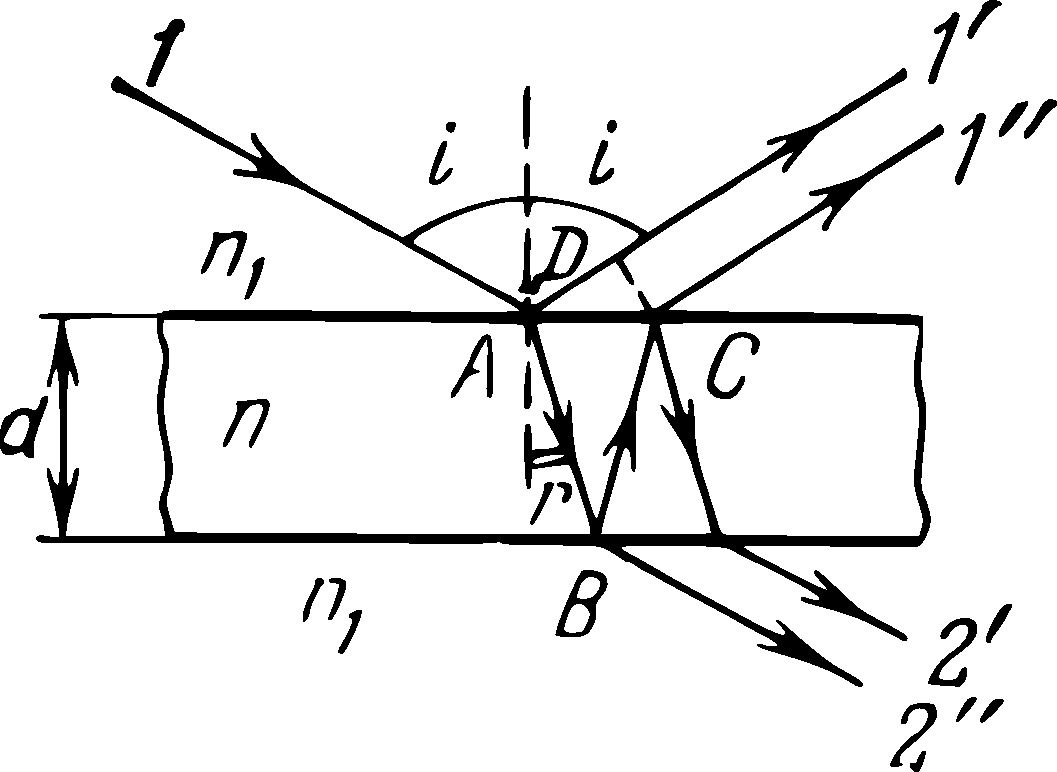
\includegraphics[width=\textwidth]{figs/ch-32/fig-32-05.pdf}
\sidecaption{Relfection and refraction of light on a plate.\zhcap{光在平板上的反射与折射。}\label{fig-32-05}}
\end{marginfigure}

\subsection{}\label{32.3.3} Assume that a plane monochromatic light wave $\mathit{1}$ is incident at the angle $i$ on a plane-parallel homogeneous plate of thickness $d$ and transparent to light (\figr{fig-32-05}). Owing to the reflection of light from the upper and lower surfaces of the plate,
two plane waves propagate in the directions of the reflected rays $\mathit{1}'$ and $\mathit{1}''$. Their optical-path difference is
\zhpar{设一束平面单色光波 $\mathit{1}$ 以入射角 $i$ 射到厚度为 $d$、两表面平行且对光透明的均匀平板上（\figr{fig-32-05}）。由于光在平板的上、下表面发生反射，两列平面波分别沿反射光线 $\mathit{1}'$ 与 $\mathit{1}''$ 的方向传播。它们的光程差为：}
\begin{equation*}%
\Delta s = n (\overline{AB} + \overline{BC}) - n_{1} \left(\overline{AD} + \frac{\lambda_{1}}{2} \right) = 2 dn \cos r - \frac{\lambda_{0}}{2}.
\end{equation*}
where $n_{1}$ and $n_{2}$ are the refractive indices of the surrounding medium and of the plate, $D$ is the foot of a perpendicular erected on ray $\mathit{1}'$ from point $C$, member $\lambda_{1}/2$ takes into account the phase difference of $\pi$ as light is reflected from point $A$ \ssect{31.5.5},\sidenote[][-2cm]{It is assumed that $i < i_{\text{Br}}$ and that $n > n_{1}$. When $n < n_{1}$, a phase difference of $\pi$ occurs upon reflection of light from point $B$ and $\Delta s = 2dn \cos r + \lambda_{0}/2$, i.e. it differs from the value of $\Delta s$ for the case when $n > n_{1}$ by $\lambda_{0}$, has no effect on the result of the interference.}
$r$ is the refractive angle, and $\lambda_{0}$ is the wavelength of the light in vacuum.
\zhpar{式中 $n_{1}$ 与 $n_{2}$ 分别为周围介质与平板的折射率，$D$ 为从点 $C$ 向反射光线 $\mathit{1}'$ 所作垂线的垂足，$\lambda_{1}/2$ 项考虑了光在点 $A$ 反射时的相位差 $\pi$（\ssect{31.5.5}），$r$ 为折射角，$\lambda_{0}$ 为光在真空中的波长。}
\zhpar{注：假定 $i < i_{\text{Br}}$（$i_{\text{Br}}$ 为布儒斯特角）且 $n > n_{1}$。若 $n < n_{1}$，则光在点 $B$ 反射时出现相位差 $\pi$，此时 $\Delta s = 2dn \cos r + \lambda_{0}/2$，它与 $n > n_{1}$ 时的 $\Delta s$ 相差 $\lambda_{0}$，这一差别对干涉结果没有影响。}

The conditions for interference maxima of reflection are
\zhpar{反射光干涉极大的条件为：}
\begin{align*}%
2dn \cos r & = (2m + 1) \frac{\lambda_{0}}{2}, \qor \\
2d \cos r & = (2m + 1) \frac{\lambda}{2},
\end{align*}
where $m = 0,\, 1,\, 2, \dots$ is the order of the interference maximum.
\zhpar{式中 $m = 0,\, 1,\, 2, \dots$ 为干涉极大的级次。}

The conditions for interference minima of reflection are
\zhpar{反射光干涉极小的条件为：}
\begin{align*}%
2dn \cos r & = m \lambda_{0}, \qor \\
2d \cos r & = m \lambda,
\end{align*}
where $m = 1,2, \dots{}$ is the order of the interference minimum.
\zhpar{式中 $m = 1,2, \dots{}$ 为干涉极小的级次。}

The optical-path difference for the waves passing through the
plate (rays $\mathit{2}'$ and $\mathit{2}''$) is $\Delta s = 2dn \cos r$, i.e. it differs from $\Delta s$ for the reflected light by $\lambda_{0}/2$. Therefore, the maxima of reflection correspond to the minima of transmission of light and vice vcra. If the plate is illuminated with white light, it has additional colouring in the reflected and transmitted light.
\zhpar{穿过平板的波（光线 $\mathit{2}'$ 与 $\mathit{2}''$）的光程差为 $\Delta s = 2dn \cos r$，它与反射光的 $\Delta s$ 相差 $\lambda_{0}/2$。因此，反射极大对应于透射极小，反之亦然。若用白光照射平板，则反射光与透射光中都会出现附加的颜色。}

The maximum thickness $d$ of the plate at which it is still possible to observe interference fringes is limited by the coherence time $\tau_{\text{coh}}$ of the light \ssect{32.1.4}. Thus
\zhpar{能够观察到干涉条纹的平板最大厚度 $d$，受光的相干时间 $\tau_{\text{coh}}$ 的限制（\ssect{32.1.4}）。于是有：}
\begin{equation*}%
2dn \cos r < c \tau_{\text{coh}} \qor 2d cos r < l_{\text{coh}},
\end{equation*}
where $l_{\text{coh}} = v \tau_{\text{coh}} = c \tau_{\text{coh}}/n$ is the coherence length.
\zhpar{式中 $l_{\text{coh}} = v \tau_{\text{coh}} = c \tau_{\text{coh}}/n$ 为相干长度。}

\subsection{}\label{32.3.4} In the calculation of the optical-path difference of interfering waves in a plate \ssect{32.3.3} only two waves were taken into account. They correspond to the first reflection from the upper and from the lower surfaces of the plate; the possibility of multiple reflection of light was neglected. Such simplification is justified only if the intensity $I_{2}$ of the wave corresponding to the second reflection from the lower surface of the plate is substantianlly less than the intensity $I_{1}$ of the wave corresponding to the first reflection. 
\zhpar{在计算平板中干涉波的光程差（\ssect{32.3.3}）时，只考虑了两束波。它们分别对应于光在平板上表面与下表面的第一次反射；光的多次反射被忽略了。只有当对应于下表面第二次反射的波的强度 $I_{2}$ 远小于对应于第一次反射的波的强度 $I_{1}$ 时，这种简化才是合理的。}


If $R$ is the coefficient of reflection \ssect{31.5.6} from
the upper and lower surfaces of the plate, then $I_{2} = R^{2}I_{1}$. As a rule $R^{2} \ll 1$. At the interface, for instance between air and glass $(n_{21} = 1.5)$, at angles
of incidence $i < \ang{50}$, the coefficient of reflection $R 
< 0.05$. In certain special cases, when $I_{2}$ is comparable
to $I_{1}$ it is necessary to deal with multiwave interference (\ref{sec-32.4}).
\zhpar{若 $R$ 为平板上、下表面的反射系数（\ssect{31.5.6}），则 $I_{2} = R^{2}I_{1}$。通常 $R^{2} \ll 1$。例如，对于空气与玻璃（$n_{21} = 1.5$）之间的界面，入射角 $i < \ang{50}$ 时，反射系数 $R < 0.05$。在某些特殊情形下，当 $I_{2}$ 与 $I_{1}$ 相当时，必须考虑多光束干涉（见 \ref{sec-32.4}）。}

\subsection{}\label{32.3.5} In considering the interference of light in thin films, distinction is made between interference fringes of equal inclination (isoclinic fringes) and those of equal thickness (isopachic fringes). \redem{Equal-inclination fringes} are observed when a diverging (or converging) beam of light is incident at various angles $i$ on a thin plane-parallel film. These, for instance, are the conditions that prevail when the film is illuminated by an extended source
or scattered sunlight. Since $d$ and $n$ are the same all over the film, the optical-path difference of the interfering waves varies along the surface of the film only owing to the variation in the angle of incidence $i$. 
\zhpar{在研究薄膜中的光干涉时，通常区分\redem{等倾干涉条纹}（等倾条纹）与\redem{等厚干涉条纹}（等厚条纹）。当发散（或会聚）光束以各种入射角 $i$ 射到薄的平行平板薄膜上时，便观察到等倾干涉条纹。例如，薄膜被扩展光源或被散射的日光照明时，就是这种情形。由于薄膜各处的 $d$ 与 $n$ 都相同，干涉波的光程差沿薄膜表面的变化，仅由入射角 $i$ 的变化引起。}
\begin{marginfigure}%[-3cm]
\centering
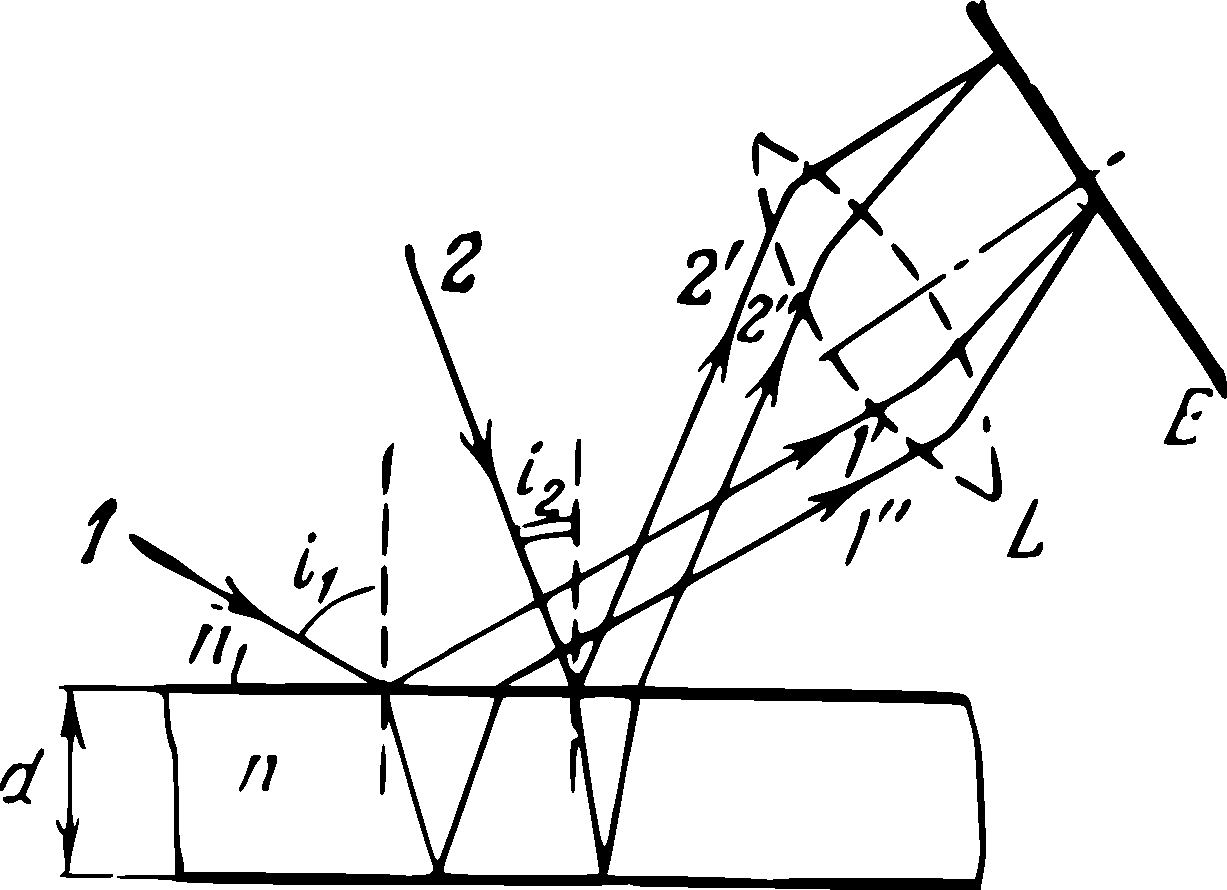
\includegraphics[width=\textwidth]{figs/ch-32/fig-32-06.pdf}
\sidecaption{The conditions for intereference for equal inclination fringes.\zhcap{等倾干涉条纹的形成条件。}\label{fig-32-06}}
\end{marginfigure}

The conditions of interference are the same for all rays incident on the surface of the film and reflected from it at the same angle. Consequently, the interference pattern in this case is said to be made up of equal-inclination fringes.
Equal-inclination fringes are observed on screen $E$ arranged in the focal plane of a convergent lens $L$ (\figr{fig-32-06}). With no lens available the interference pattern could only be observed at infinity, at the point of intersection of the parallel rays $\mathit{1}'$ and $\mathit{1}''$, $\mathit{2}'$,  and $\mathit{2}''$ etc. Therefore, equal-inclination fringes are said to be localized at infinity. For their visual observation it would be necessary for the eyes to accommodate to infinity.
\zhpar{对于以相同角度射到薄膜表面并从其上反射的所有光线，干涉条件都相同。因此，这种情形下的干涉图样称为由等倾干涉条纹组成。等倾干涉条纹被观察于置于会聚透镜 $L$ 焦平面上的屏 $E$ 上（\figr{fig-32-06}）。若没有透镜，干涉图样只能在无穷远处观察到，即在平行光线 $\mathit{1}'$ 与 $\mathit{1}''$、$\mathit{2}'$ 与 $\mathit{2}''$ 等相交之处。因此，等倾干涉条纹称为定域于无穷远。要用眼睛直接观察它们，眼睛需要调节到无穷远。}

\subsection{}\label{32.3.6} \redem{Equal-thickness fringes} are observed in reflecting a parallel or almost parallel beam of light rays ($i$ = const.) from a thin transparent film whose thickness $d$ is not the same at various places. The optical-path difference of the interfering waves varies in going from certain points on the surface of the film to other points with a corresponding change in the film thickness $d$. Hence the conditions of interference are the same for points having
the same values of $d$. This is why the interference pattern being considered is said to he made up of equal-thickness fringes. Equal-thickness fringes are localized close to the surface of the film. Hence, they can he observed
by accommodation of the eyes practically
to the film's surface.
\zhpar{当平行或近似平行的光线（$i$ = 常量）从厚度 $d$ 各处不同的透明薄膜上反射时，便观察到\redem{等厚干涉条纹}。当沿薄膜表面从一点移动到另一点时，干涉波的光程差随膜厚 $d$ 的相应变化而变化。因此，对于 $d$ 值相同的各点，干涉条件相同。所以，这种干涉图样称为由等厚干涉条纹组成。等厚干涉条纹定域于薄膜表面附近，因此实际上只需使眼睛几乎调节到薄膜表面，即可对其进行观察。}

When light interferes in a thin transparent wedge with a small wedge angle $\alpha$, equal-thickness fringes have the form of straight hands parallel to the edge of the wedge. If the wedge
is illuminated by monochromatic light with the wavelength $\lambda_{0}$ in vacuum, normally incident on the wedge surface
$(i = 0)$, the width of the interference fringes \ssect{32.2.3} is equal to $\lambda_{0}/2n\alpha$, where $n$ is the absolute refractive index of the wedge material.
\zhpar{当光在楔角 $\alpha$ 很小的透明薄楔形膜中发生干涉时，等厚干涉条纹呈与楔棱平行的直条纹。若以真空中波长为 $\lambda_{0}$ 的单色光垂直入射到楔面上（$(i = 0)$），则干涉条纹的宽度（\ssect{32.2.3}）等于 $\lambda_{0}/2n\alpha$，其中 $n$ 为楔形材料的绝对折射率。}

\begin{marginfigure}%[-3cm]
\centering
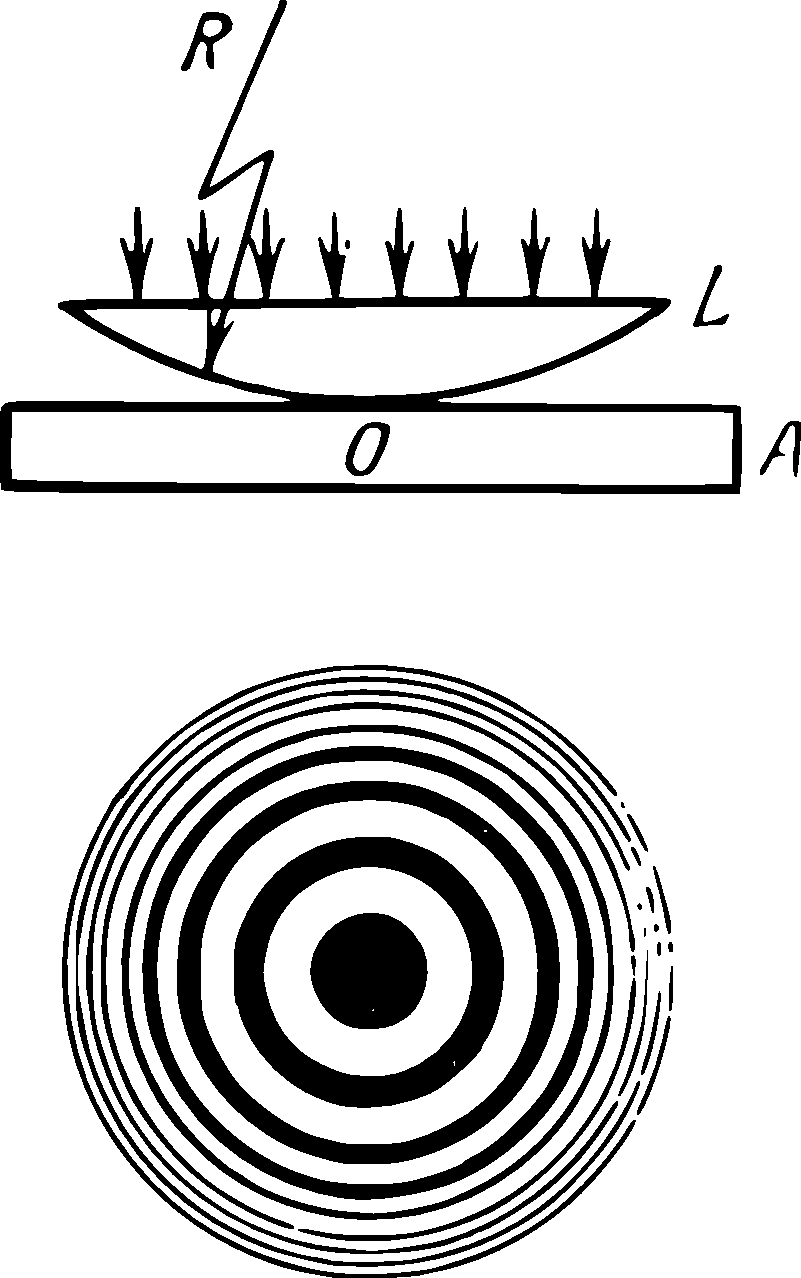
\includegraphics[width=0.9\textwidth]{figs/ch-32/fig-32-07.pdf}
\sidecaption{Newton's rings are fringes of equal thickness.\zhcap{牛顿环是等厚干涉条纹。}\label{fig-32-07}}
\end{marginfigure}
\subsection{}\label{32.3.7} Equal-thickness fringes having the form of concentric rings, and called \redem{Newton's rings}, are observed in the interference of light in the thin
air clearance between a flat glass plate $A$ and a flat-convex lens $L$ pressed tightly against the plate (\figr{fig-32-07}). The flat surface of the lens is parallel to the plate
surface and light is normally incident to the lens surface. The centre of Newton's rings coincides with point $O$ of contact between the lens and plate. At a small distance $r$ from point $O$ the optical-path difference of the waves reflected from the upper and lower surfaces of the nir clearance is 
\zhpar{等厚干涉条纹呈同心圆环状，称为\redem{牛顿环}。它是在紧压于平板玻璃 $A$ 上的平凸透镜 $L$ 与平板之间的薄空气层中观察到的光干涉现象（\figr{fig-32-07}）。透镜的平面与玻璃平板表面平行，光垂直入射到透镜表面上。牛顿环的中心与透镜和平板的接触点 $O$ 重合。在距点 $O$ 为小距离 $r$ 处，从空气层上、下表面反射的两束波的光程差为：}
\begin{equation*}%
\Delta s \approx n \frac{r^{2}}{R} + \frac{\lambda_{0}}{2},
\end{equation*}
where $n \approx 1$ (for air), and $R$ is the radius of the convex surface on the lens.
\zhpar{式中 $n \approx 1$（对于空气），$R$ 为透镜凸球面的半径。}


\textbf{Note.} In calculations concerning Newton's rings, the wave reflected from the upper (flat) surface of the lens need not be taken into account because the optical-path difference between this wave and the waves reflected from the boundaries of the air clearance is greater than the coherence length for nonlaser light \ssect{32.3.3}.
\zhpar{\textbf{注意：}在计算牛顿环时，无需考虑从透镜平面（上表面）反射的波，因为该波与从空气层边界反射的波之间的光程差大于非激光光源的相干长度（\ssect{32.3.3}）。}

In reflected monochromatic light with the wavelength in air
$\lambda = \lambda_{0} /n  \approx \lambda_{0}$, the radii of the dark and bright Newton's rings are
\zhpar{在空气中波长为 $\lambda = \lambda_{0} /n \approx \lambda_{0}$ 的反射单色光中，暗环与亮环的半径分别为：}
\begin{align*}%
r_{\text{dark}} & = \sqrt{m R \lambda } \qand \\
r_{\text{bright}} & = \sqrt{(2m + 1) \frac{R \lambda }{2}},
\end{align*}
where $m = 0, 1, 2, \dots{}$. The dark spot in the centre of the pattern corresponds to the change in the phase of the wave by $\pi$ when it is reflected from the lower surface of the air clearance.
\zhpar{式中 $m = 0, 1, 2, \dots{}$。图样中心的暗斑对应于光在空气层下表面反射时相位改变了 $\pi$。}

If white light is incident on the lens, a central dark spot
is observed in the reflected light, surrounded by a system of coloured rings. These rings correspond to the interference maxima of the reflection of light with various values
of wavelength $\lambda$.
\zhpar{若以白光照射透镜，则在反射光中观察到中心为暗斑、周围环绕一系列彩色圆环的图样。这些圆环对应于不同波长 $\lambda$ 的光反射后的干涉极大。}

\begin{marginfigure}[-2cm]
\centering
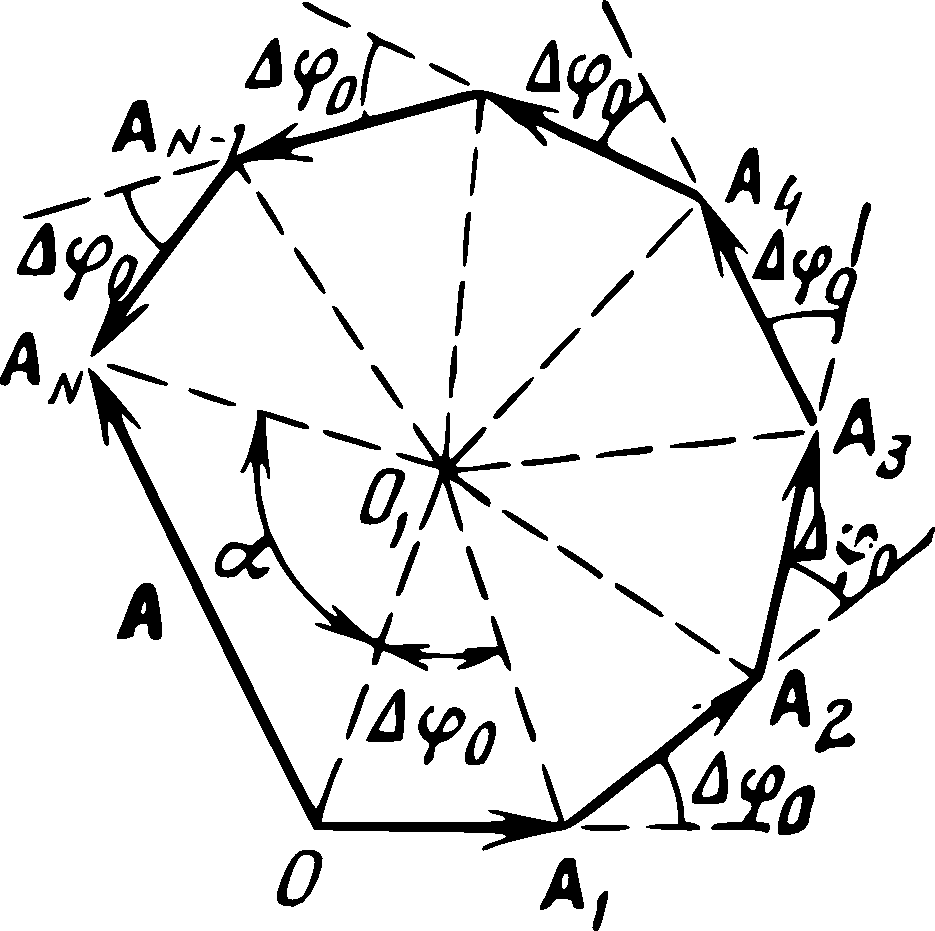
\includegraphics[width=\textwidth]{figs/ch-32/fig-32-08.pdf}
\sidecaption{Analysing interferene of multiple waves.\zhcap{多光束干涉的分析。}\label{fig-32-08}}
\end{marginfigure}
\section{Multiwave Interference}
\label{sec-32.4}
\zhtitle{多光束干涉}


\subsection{}\label{32.4.1} Special interference instruments,
such as the diffraction grating \ssect{33.3.4}, the Fabry-Perot etalon and others are used to obtain interference of many light waves with close or equal amplitudes. The amplitude $A$ of the resultant vibration and its intensity $I = A^{2}$ at arbitrary point $M$ can be found by applying the method of vector diagrams for adding oscillations or vibrations
having the same direction \ssect{28.4.2}.
\zhpar{利用衍射光栅（\ssect{33.3.4}）、法布里-珀罗标准具等专用干涉仪器，可以获得许多振幅相近或相等的光波的干涉。在任意点 $M$ 处，合振动的振幅 $A$ 及其强度 $I = A^{2}$，可用同方向振动合成的矢量图解法求得（\ssect{28.4.2}）。}


\subsection{}\label{32.4.2} Shown in \figr{fig-32-08} is a vector diagram of the addition of vibrations in interference of $N$ waves. At the point $M$ being considered, these vibrations set up coherent vibrations in the same direction with equal amplitudes $A_{i} = A_{1}$ and a phase difference, independent of $i$, between $(i + 1)$-th and $i$-th vibrations. Thus $\Phi_{i+1} (t) - \Phi_{i} (t) = \Delta \varphi_{0}$. The amplitude of the resultant vibration is
\zhpar{\figr{fig-32-08}给出了 $N$ 个波干涉时振动合成的矢量图。在所考察的点 $M$ 处，这些振动激发出同方向的相干振动，各振幅相等，$A_{i} = A_{1}$，且第 $(i + 1)$ 次与第 $i$ 次振动之间的相位差与 $i$ 无关。即 $\Phi_{i+1} (t) - \Phi_{i} (t) = \Delta \varphi_{0}$。合振动的振幅为：}
\begin{equation*}
A = 2 \times \seg{OO}_{1} \abs{\sin \frac{\alpha}{2}},
\end{equation*}
where 
\zhpar{其中：}
\[
\alpha = 2\pi - N \Delta \varphi_{0}, \qand \seg{OO}_{1} = \frac{A_{1}}{2 \abs{\sin \dfrac{\Delta \varphi_{0}}{2}}}.
\]
Hence,
\zhpar{由此得：}
\begin{equation*}
A = A_{1} \abs{\frac{\sin \dfrac{N \Delta \varphi_{0}}{2}}{\sin \dfrac{\Delta \varphi_{0}}{2}}}, \qand  I = I_{1} \frac{\sin^{2} \dfrac{N \Delta \varphi_{0}}{2}}{\sin^{2} \dfrac{\Delta \varphi_{0}}{2}}.
\end{equation*}
where $I_{1} = A_{1}^{2}$ is the intensity of the vibration set up at point $M$ by each of the $N$ interfering waves separately.
\zhpar{式中 $I_{1} = A_{1}^{2}$ 为每个干涉波单独在点 $M$ 处激发的振动强度。}

\begin{figure}%[-3cm]
\centering
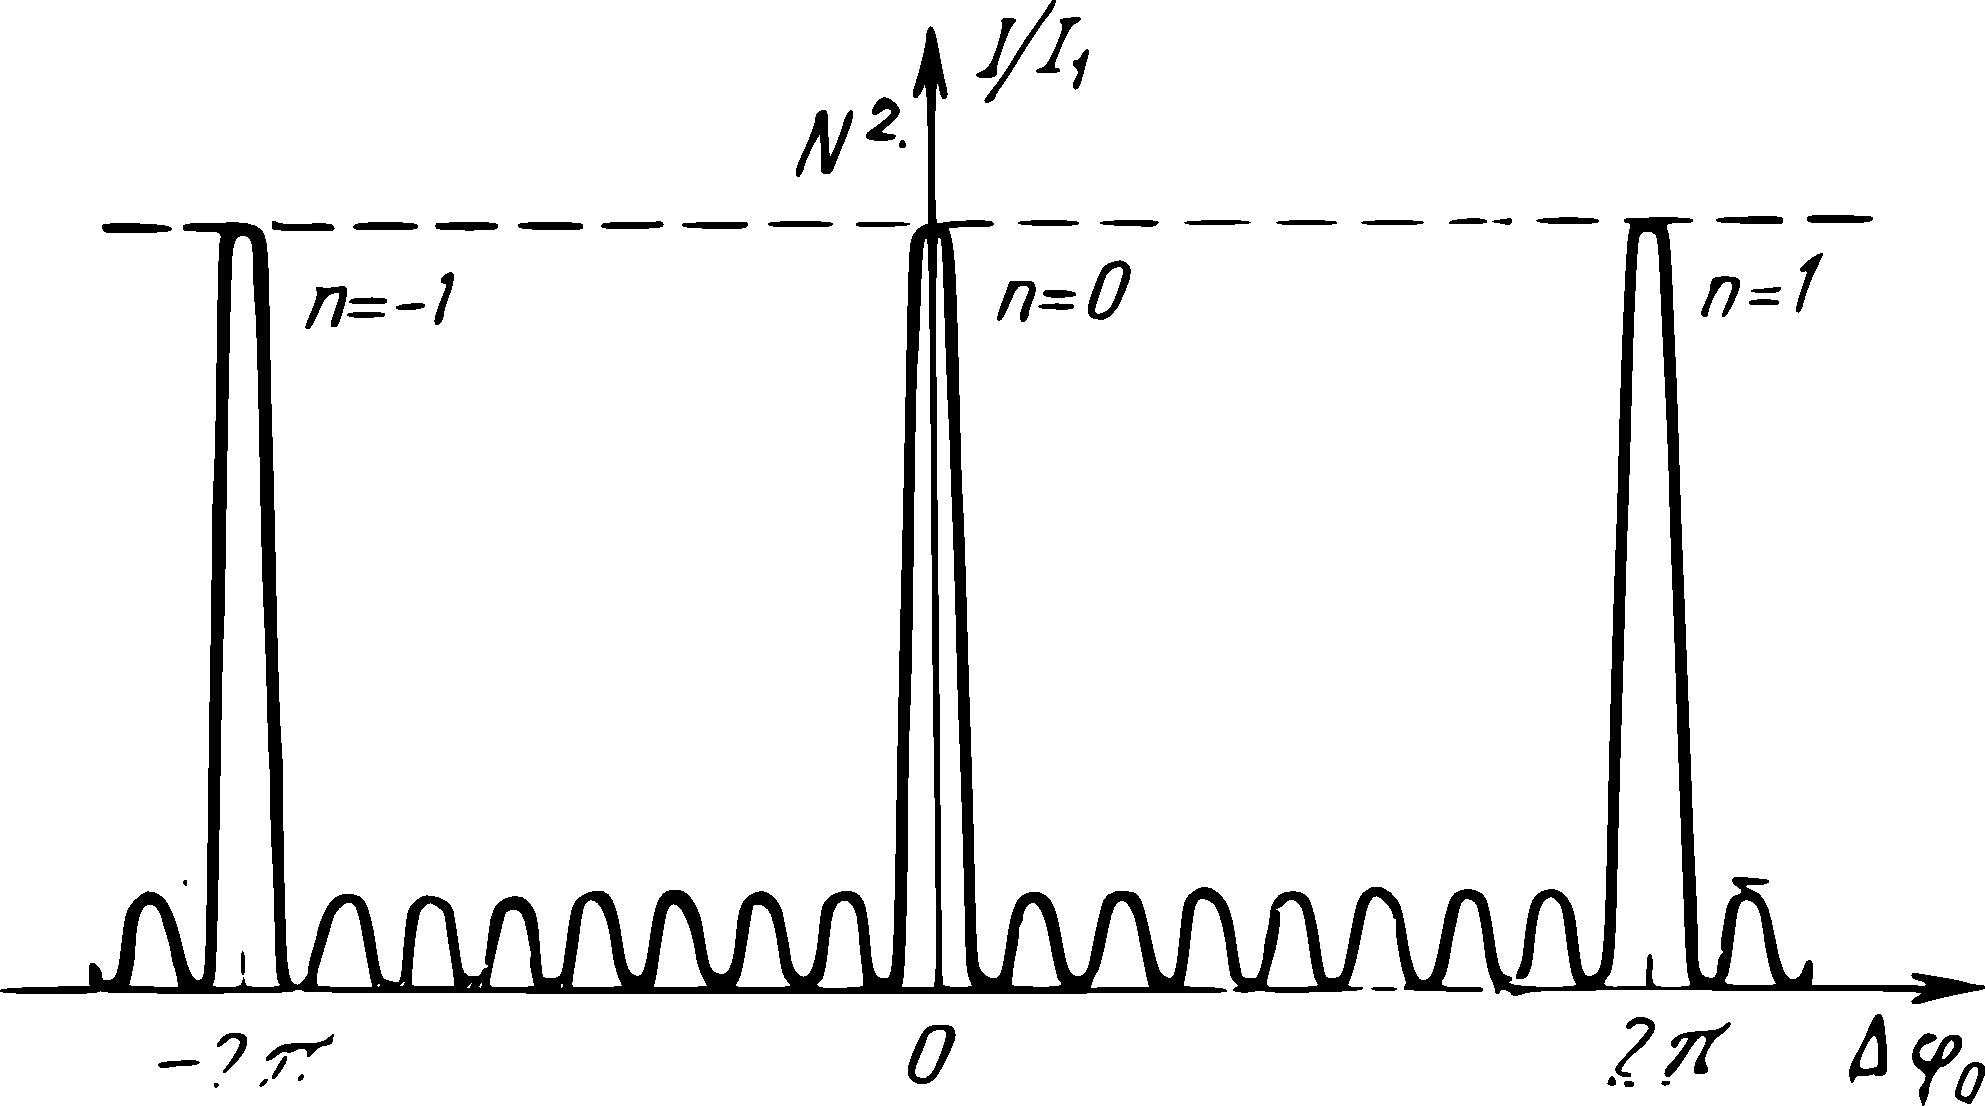
\includegraphics[width=\textwidth]{figs/ch-32/fig-32-09.pdf}
\sidecaption{The nature of the dependence of $I/I_{1}$ on $\Delta \varphi_{0}$. \zhcap{$I/I_{1}$ 随 $\Delta \varphi_{0}$ 的变化特性。}\label{fig-32-09}}
\end{figure}

\subsection{}\label{32.4.3} The \redem{principal maxima in the interference} of $N$ waves \ssect{32.4.2} are at points $M$ that comply with the condition: $\Delta (\varphi_{0} = \pm 2n \pi$ where $n = 0, \,1,\, 2, \dots{}$ is the \redem{order of the principal maximum}. The amplitude and intensity of vibration at the principal maxima are:
\zhpar{$N$ 个波干涉的\redem{主极大}（\ssect{32.4.2}）位于满足下列条件的点 $M$ 处：$\Delta (\varphi_{0} = \pm 2n \pi$，其中 $n = 0, 1, 2, \dots{}$ 为\redem{主极大的级次}。主极大处振动的振幅与强度分别为：}
\begin{equation*}%
A_{\text{max}} =  NA_{1} \qand I_{\text{max}} = N^{2}I_{1}.
\end{equation*}
\redem{Interference minima} $(A = 0)$ comply with the condition:
\zhpar{干涉极小（$A = 0$）满足下列条件：}
\begin{equation*}%
\Delta \varphi_{0} = \pm 2\pi \frac{p}{N}, 
\end{equation*}
where $p$ may be any positive whole number except a multiple of $N$.
\zhpar{式中 $p$ 可以是任意正整数，但不能是 $N$ 的整数倍。}

The nature of the dependence of $I/I_{1}$ on $\Delta \varphi_{0}$ \ssect{32.4.2} is shown in \figr{fig-32-09}. Between each pair of adjacent interference minima there is a maximum, either a principal or a subordinate maximum. At high $N$ values the intensities of the subordinate maxima
are negligibly small compared to that of the principal maxima.
The values $\Delta \varphi_{0} = \pm (2\pi n \pm 2\pi/N)$ correspond to two minima that bound a principal maximum of the $n$-th. order. Therefore, the ``width'' of the principal maximum, equal to $4\pi/N$, is inversely proportional to the number N of interfering waves, and its intensity is proportional to $A^{2}$. 
\zhpar{$I/I_{1}$ 随 $\Delta \varphi_{0}$ 的变化特性（\ssect{32.4.2}）如\figr{fig-32-09}所示。相邻两个干涉极小之间都有一个极大，它可以是主极大，也可以是次极大。当 $N$ 很大时，次极大的强度与主极大相比可以忽略不计。$\Delta \varphi_{0} = \pm (2\pi n \pm 2\pi/N)$ 对应于限定第 $n$ 级主极大的两个极小。因此，主极大的“宽度”等于 $4\pi/N$，与干涉波数 $N$ 成反比，而其强度与 $A^{2}$ 成正比。}

The  fact that the interference pattern changes in such a manner as $N$ is varied fully complies with the law of conservation of energy. The total energy of vibration at all points of the screen on which the interference pattern is observed is proportional to $N$.
\zhpar{随 $N$ 改变，干涉图样呈现的这种变化完全符合能量守恒定律。在观察干涉图样的整个屏上，各点振动的总能量与 $N$ 成正比。}

\begin{marginfigure}[-2cm]
%\centering
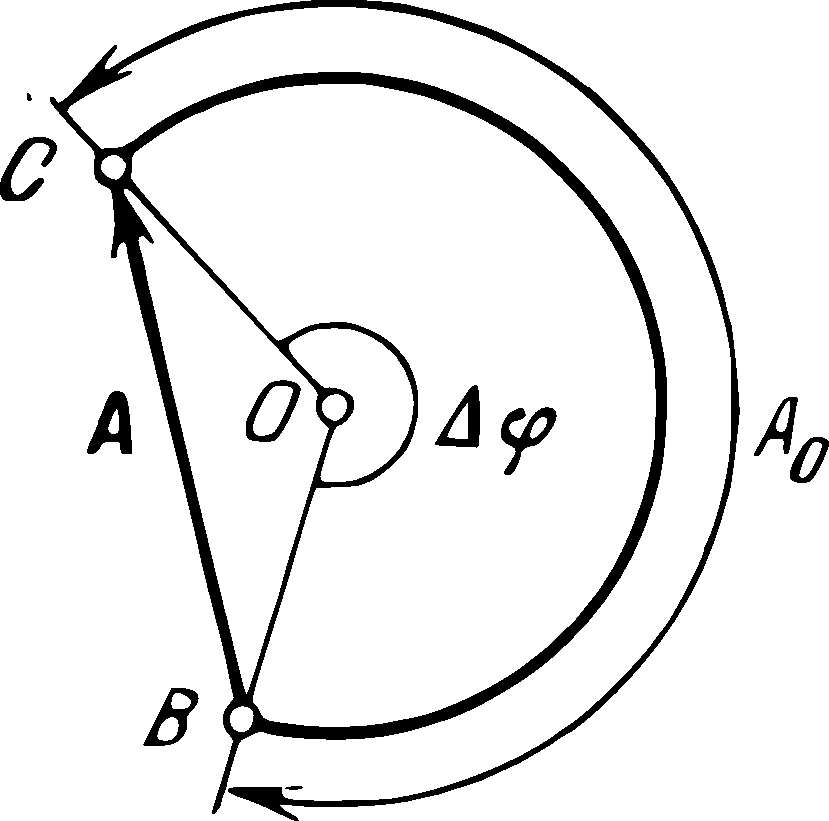
\includegraphics[width=0.8\textwidth]{figs/ch-32/fig-32-10.pdf}
\sidecaption{Form of \figr{fig-32-10} when number of interfering waves is increased indefinitely. \zhcap{干涉波数无限增加时\figr{fig-32-10}的形状。}\label{fig-32-10}}
\end{marginfigure}


\subsection{}\label{32.4.4} If the number $N$ of interfering waves \ssect{32.4.2} is increased indefinitely, and their amplitudes $A_{1}$ and phase differences $\Delta \varphi_{0}$ are correspondingly reduced so that $N A_{1}$ and $N \Delta \varphi_{0}$ remain finite quantities equal to $A_{0}$ and $\Delta \varphi_{0}$, then, in the limit, the vector diagram (\figr{fig-32-08}) assumes the form illustrated in \figr{fig-32-10}. Vector $A$, the amplitude of the resultant vibration, closes the arc $BC$ of a circle. The length of this arc is equal to $A_{0}$ and its central angle $\angle BOC = \Delta \varphi$. Therefore, the radius of the circle $\overline{OB} = A_{0}/\Delta  \varphi$, and the amplitude $A$ and intensity $I$ of the resultant vibration equal
\zhpar{若干涉波的数目 $N$ 无限增大，同时使各波的振幅 $A_{1}$ 与相位差 $\Delta \varphi_{0}$ 相应减小，使 $NA_{1}$ 与 $N\Delta \varphi_{0}$ 保持为有限值，分别等于 $A_{0}$ 与 $\Delta \varphi_{0}$，那么在极限情形下，矢量图（\figr{fig-32-08}）将具有\figr{fig-32-10}所示的形式。表示合振动振幅的矢量 $A$ 封闭了一段圆弧 $BC$。该圆弧的长度等于 $A_{0}$，其圆心角 $\angle BOC = \Delta \varphi$。因此，圆的半径 $\overline{OB} = A_{0}/\Delta \varphi$，合振动的振幅 $A$ 与强度 $I$ 分别为：}
\begin{equation*}%
A = A_{0} \abs{\frac{\sin \dfrac{\Delta \varphi}{2}}{ \dfrac{\Delta \varphi}{2}}}, \qand  I = I_{0} \frac{\sin^{2} \dfrac{ \Delta \varphi}{2}}{ \left( \dfrac{\Delta \varphi}{2} \right)^{2}}.
\end{equation*}
where $I_{0} = A_{0}^{2}$.
\zhpar{式中 $I_{0} = A_{0}^{2}$。}

\redem{Interference minima} are at points of the interference pattern for which
\zhpar{\redem{干涉极小}位于干涉图样中满足下列条件的点：}
\begin{equation*}%
\Delta \varphi = \pm 2m \pi,
\end{equation*}
where $m = 1,\, 2, \, \dots{}$.
\zhpar{式中 $m = 1,\, 2, \, \dots{}$。}


\begin{figure}%[-3cm]
%\centering
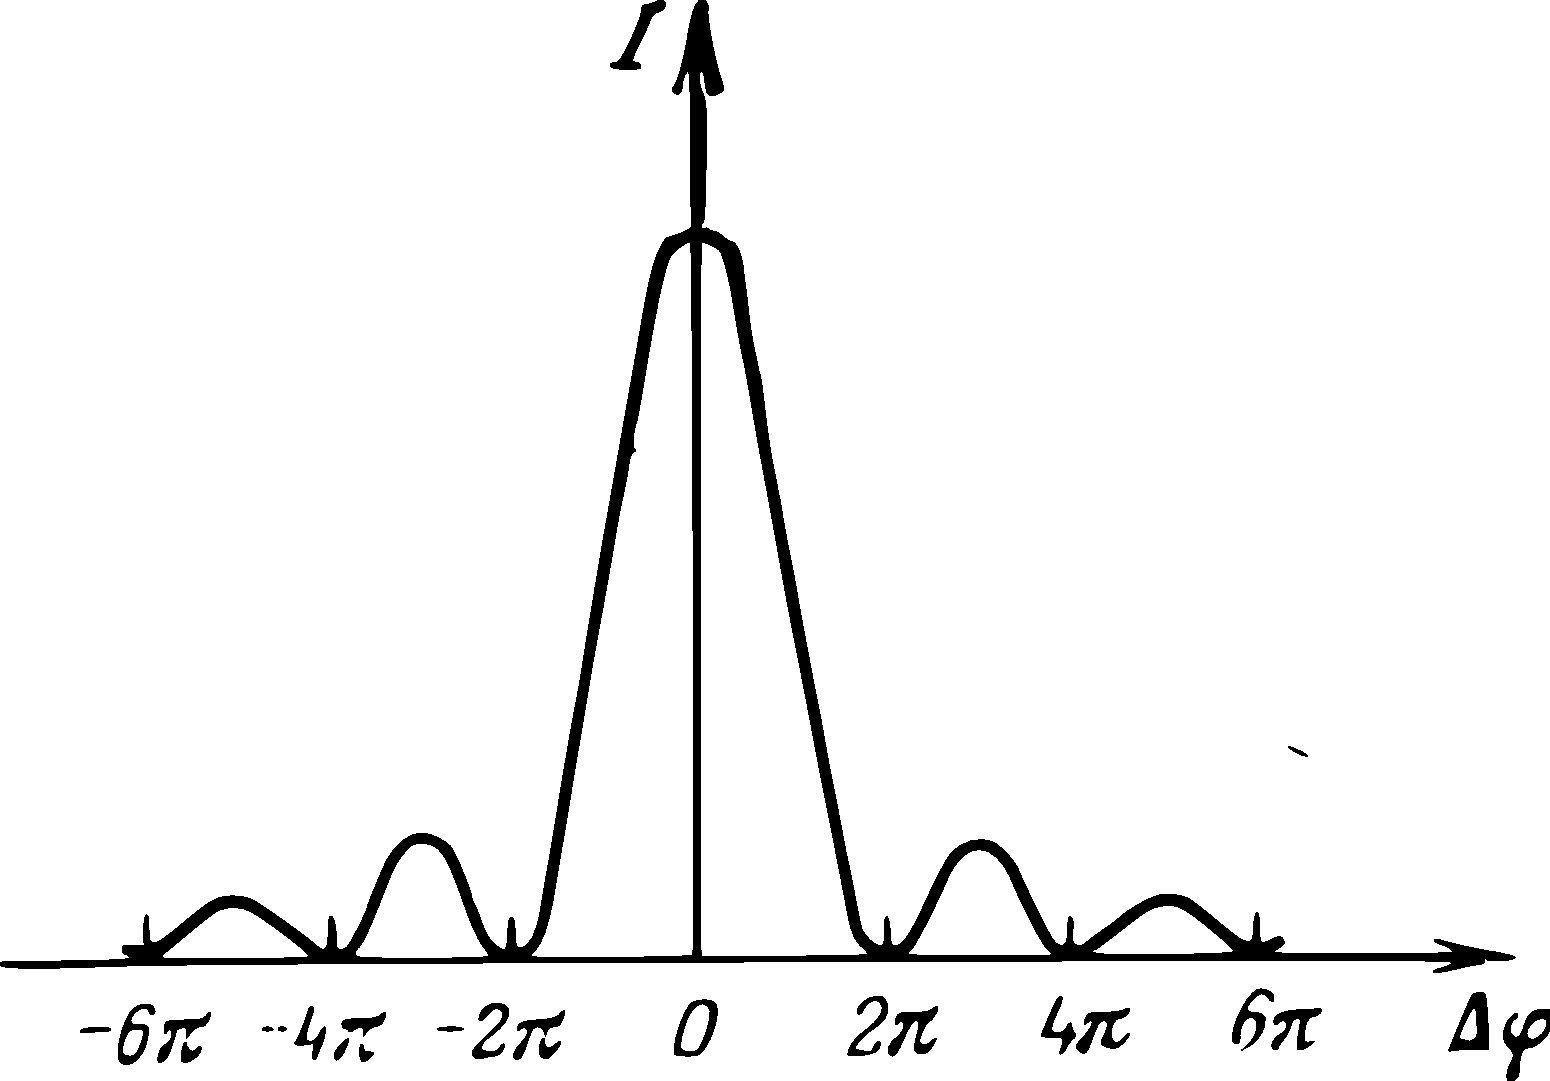
\includegraphics[width=0.8\textwidth]{figs/ch-32/fig-32-11.pdf}
\sidecaption{The dependence of $I$ on $\Delta \varphi_{0}$. \zhcap{$I$ 随 $\Delta \varphi_{0}$ 的变化关系。}\label{fig-32-11}}
\end{figure}

\redem{Interference maxima} are at points for which \begin{equation*}%
\Delta \varphi = \pm 2 k_{m} \pi,
\end{equation*}
\zhpar{\redem{干涉极大}位于满足下式的点上：}
where $m = 1,\, 2, \, \dots{}$ is the \redem{order of the maximum}. The values of factor $k_{m}$ are determined from the transcendental equation $\tan k_{m} \pi = k_{m} \pi$. For the central, zero-order maximum $k_{0} = 0$ and $\Delta \varphi_{0}$. The amplitude and intensity of vibration at a zero-order maximum are equal to $A_{0}$ and $I_{0}$. For all other maxima $(m \geqslant 1)$ it can be assumed approximately that 
\zhpar{式中 $m = 1,\, 2, \, \dots{}$ 为\redem{极大的级次}。因子 $k_{m}$ 的值由超越方程 $\tan k_{m} \pi = k_{m} \pi$ 确定。对于中央的零级极大，$k_{0} = 0$，并有 $\Delta \varphi_{0}$。零级极大处振动的振幅与强度分别等于 $A_{0}$ 与 $I_{0}$。对于其他所有极大（$m \geqslant 1$），可以近似地认为：}
\begin{equation*}%
k_{m} = \frac{(2m + l)}{2} \qand \Delta \varphi = \pm (2m + 1) \pi.
\end{equation*}
Accordingly, the ratio of the intensities for the $m$-th and zero-order maxima equals
\zhpar{因此，第 $m$ 级与零级极大的强度之比为：}
\begin{equation*}%
\frac{I_{m}}{I_{0}} = \frac{4}{(2m + 1)^{2}\pi^{2}}.
\end{equation*}

\begin{table}
\centering
\begin{tabular}{p{2cm}ccccc}
\toprule
\textbf{Order of the maximum} & \textbf{0} & \textbf{1} & \textbf{2} & \textbf{3} & \textbf{4}\\
\midrule
$I_{m}/ I_{0}$ & 1 0.045 & 0.016 & 0.008 &   0.005 \\
\bottomrule
\end{tabular}
\sidecaption{Intensity of $m$-th and 0-th order maximum as a function of order. \zhcap{$m$ 级与零级极大的强度随级次的变化。}\label{tab-32-01}}
\end{table}
This ratio decreases rapidly with an increase of $m$ (\tabl{tab-32-01}). The shape of the curve showing the dependence of $I$ on $\Delta \varphi_{0}$ is
shown in \figr{fig-32-11}.
\zhpar{该比值随 $m$ 的增大而迅速减小（\tabl{tab-32-01}）。$I$ 随 $\Delta \varphi_{0}$ 变化的曲线形状如\figr{fig-32-11}所示。}

